\section{Part III. Integration}
%
%\begin{mdframed}[backgroundcolor=paleyellow,linewidth=1pt]
%\begin{center}
%{\sc\Large Part III. Integration}
%\end{center}
%\end{mdframed}
\lecmargin{19}
We now want to develop a theory of integration of complex-valued functions in a single complex variable. Integrals will be defined over suitable curves (contours) in the complex plane. This theory of integration is a surprisingly powerful tool in the study of holomorphic functions.\\
\\
Using this theory, we will obtain powerful characterisations of holomorphic functions. Roughly speaking we will prove the following: let $G$ be a domain and $f:G \to \cc$ a function. The following are equivalent. 
\begin{itemize}
\item[(1)] $f$ is holomorphic on $G$.
\item[(2)] For all $n \in \zz_{>0}$, $f^{(n)}$ exists and is holomorphic on $G$.
\item[(3)] In each \emph{simply connected} subdomain $D$ of $G$, there exists a holomorphic function $F:D \to \cc$ such that $F' = f\vert_D$. 
\item[(4)] $f$ is continuous on $G$ and 
\[\int_C f(z)\,dz = 0\]
for every \emph{contour} $C$ lying in a \emph{simply connected} subdomain.
\item[(5)] If $C$ is a \emph{simple closed contour} in $G$ and $z_0$ is interior to $C$, then
\[f'(z_0) = \frac{1}{2\pi i}\int_C \frac{f(z)}{z - z_0}\,dz.\]
\end{itemize}
Additionally, as an application of the theory, we will prove
\begin{itemize}
\item \emph{Liouville's theorem}. Every bounded holomorphic function is constant.
\item \emph{Fundamental Theorem of Algebra}. Every polynomial of degree $n \geq 1$ has atleast one complex root.
\end{itemize}

\medskip

\subsection{Derivatives of Functions of a Real-variable}
%\begin{mdframed}
%\begin{center}
%{\Large Derivatives of Functions of a Real-variable}
%\end{center}
%\end{mdframed}
To define an integral of a complex-valued functions in a single complex variable, we need to understand how to differentiate a complex-valued function in a single real variable
\[\gamma: [a,b] \to \cc,\]
where $[a,b] \subseteq \rr$.

\medskip

\begin{definition}
For $\gamma:[a,b] \to \cc$, writing $\gamma(t) = u(t) + i\,v(t)$, where $u,\,v:[a,b] \to \rr$, we define the \emph{derivative} of $\gamma$ to be
\[\gamma'(t) = u'(t) + iv'(t),\]
provided that $u'(t)$ and $v'(t)$ exist. In this case, we say $\gamma$ is differentiable.
\end{definition}

\medskip

\begin{proposition}
Suppose $\gamma_1(t) = u_1(t) + iv_1(t)$ and $\gamma_2(t) = u_2(t) + iv_2(t)$ are differentiable, then
\begin{itemize}
\item[(1)] $(\gamma_1 + \gamma_2)'(t) = \gamma_1'(t) + \gamma_2'(t)$
\item[(2)] $(\gamma_1\gamma_2)'(t) = \gamma_1'(t)\gamma_2(t) + \gamma_1(t)\gamma_2'(t)$
\end{itemize}
\end{proposition}
\begin{proof}\hfill
\begin{itemize}[itemsep=1em]
\item[(1)] 
$\begin{aligned}[t]
(\gamma_1 + \gamma_2)' &=  ((u_1 + u_2) + i(v_1 + v_2))'\\[0.5em]
&= (u_1 + u_2)' + i(v_1 + v_2)'\\[0.5em]
&= (u_1' + u_2') + i(v_1' + v_2')\\[0.5em]
&= (u_1' + iv_1') + (u_2' + iv_2') = \gamma_1' + \gamma_2'
\end{aligned}$

\item[(2)] 
$\begin{aligned}[t]
(\gamma_1\gamma_2)' &=  ((u_1 + iv_1)(u_2 + iv_2))'\\[0.5em]
&=  ((u_1u_2 - v_1v_2) + i(u_1v_2 + u_2v_1))'\\[0.5em]
&= (u_1u_2 - v_1v_2)' + i(u_1v_2 + u_2v_1)'\\[0.5em]
&= (u_1u_2)' - (v_1v_2)' + i(u_1v_2)' + i(u_2v_1)'\\[0.5em]
&= (u_1'u_2 + u_1u_2') - (v_1'v_2 + v_1v_2') + i(u_1'v_2 + u_1v_2') + i(u_2'v_1 + u_2v_1')\\[0.5em]
&= (u_1'u_2 - v_1'v_2) + i(u_1'v_2 + u_2v_1') + (u_1u_2' - v_1v_2') + i(u_1v_2' + u_2'v_1)\\[0.5em]
&= (u_1' + iv_1')(u_2 + iv_2) + (u_1 + iv_1)(u_2' + iv_2')\\[0.5em]
&= \gamma_1'\gamma_2 + \gamma_1\gamma_2'
\end{aligned}$
\end{itemize}
\vspace*{-\baselineskip}
\end{proof}

\medskip

\begin{example}
We will often encounter the function $\gamma:[a,b] \to \cc$, where
\[\gamma(t) = e^{z_0t},\quad z_0 \in \cc\]
Let's compute $\gamma'(t)$, for which we first need to express it as $u(t) + iv(t)$. Let $z_0 = x_0 + iy_0$,
\begin{align*}
\gamma(t) = e^{z_0t} &= e^{(x_0 + iy_0)t}\\[0.5em]
&= e^{x_0t + iy_0t}\\[0.5em]
&= e^{x_0t}e^{iy_0t} = e^{x_0t}(\cos(y_0t) + i\sin(y_0t))
\end{align*}
Therefore, $u(t) = e^{x_0t}\cos(y_0t)$ and $v(t) = e^{x_0t}\sin(y_0t)$. We note,
\begin{align*}
u'(t) &= (e^{x_0t})'(\cos(y_0t)) + (e^{x_0t})(\cos(y_0t))' & v'(t) &= (e^{x_0t})'(\sin(y_0t)) + (e^{x_0t})(\sin(y_0t))'\\[0.5em]
 &= x_0e^{x_0t}\cos(y_0t) - y_0e^{x_0t}\sin(y_0t) & &= x_0e^{x_0t}\sin(y_0t) + y_0e^{x_0t}\cos(y_0t)
\end{align*}
Hence, 
\begin{align*}
\gamma'(t) = u'(t) + iv'(t) &= x_0e^{x_0t}\cos(y_0t) - y_0e^{x_0t}\sin(y_0t) + ix_0e^{x_0t}\sin(y_0t) + iy_0e^{x_0t}\cos(y_0t)\\[0.5em]
&= x_0e^{x_0t}(\cos(y_0t) + i\sin(y_0t)) + iy_0e^{x_0t}(\cos(y_0t) + i\sin(y_0t))\\[0.5em]
&= (x_0e^{x_0t} + iy_0e^{x_0t})(\cos(y_0t) + i\sin(y_0t))\\[0.5em]
&= (x_0 + iy_0)e^{x_0t}e^{iy_0t}\\[0.5em]
&= z_0e^{z_0t}
\end{align*}
To summarise, for $\gamma(t) = e^{z_0t}$, we have $\gamma'(t) = z_0e^{z_0t}$.
\end{example}

\bigskip

\subsection{Integral of $\gamma:[a,b] \to \cc$}
%\begin{mdframed}
%\begin{center}
%{\Large Integral of $\gamma:[a,b] \to \cc$}
%\end{center}
%\end{mdframed}

\begin{definition}[Definite Integral of $\gamma$]
Consider a function $\gamma:[a,b] \to \cc$ with \[\gamma(t) = u(t) + iv(t),\] where $u,\,v: [a,b] \to \rr$. The \cdef{definite\ integral\ of} {\color{darkred}$\gamma$} is defined as
\[\int_a^b\gamma(t)\ dt \coloneqq \int_a^bu(t)\ dt + i\int_a^bv(t)\ dt\]
provided the integrals of $u$ and $v$ exist.\\
\\
Improper integrals can be defined in a similar manner.
\end{definition}

\medskip

\begin{example}
We illustrate this definition by integrating $\gamma(t) = e^{it}$ on $[0,\pi]$.
\begin{align*}
\int_0^\pi e^{it}\ dt &= \int_0^\pi\cos t\ dt + \int_0^\pi\sin t\ dt\\[1em]
&= \Big[\sin t\,\Big]_0^\pi + i\Big[-\cos t\,\Big]_0^\pi\\[1em]
&= (\sin \pi - \sin 0) + i(-\cos\pi + \cos 0)\\[0.5em]
&= 2i
\end{align*}
\end{example}

\medskip

\begin{definition}[Piecewise Continuity]
A function $u:[a,b] \to \rr$ is \cdef{piecewise\ continuous\ on} {\color{darkred}$[a,b]$} if it is continuous on $[a,b]$ except at a finite number of points, where despite its discontinuity on those points, both one sided limits exist.\\
\\
We call $\gamma(t) = u(t) + iv(t)$ \emph{piecewise continuous} if both $u$ and $v$ are. 
\end{definition}

\medskip

\begin{remark}
The existence of the integrals 
\[\int_a^bu(t)\ dt \quad \text{and} \quad \int_a^b v(t)\ dt\]
is guaranteed when $\gamma$ is piecewise continuous.
\end{remark}

\medskip

\begin{proposition}[Properties of the Integral of $\gamma$]\label{paraint}
Suppose $\gamma$ and $\gamma_1$ are piecewise continuous on $[a,b]$, then
\begin{itemize}[itemsep=0.5em]
\item[(1)] $\displaystyle \int_a^bz_0 \gamma(t)\ dt = z_0\int_a^b\gamma(t)\ dt$, for any $z_0 \in \cc$.
\item[(2)] $\displaystyle \int_a^b \gamma(t) + \gamma_1(t)\ dt = \int_a^b\gamma(t)\ dt + \int_a^b\gamma_1(t)\ dt$.
\item[(3)] $\displaystyle \int_a^b \gamma(t)\ dt = \int_a^c\gamma(t)\ dt + \int_c^b\gamma(t)\ dt$, for any $c \in [a,b]$.
\item[(4)] $\displaystyle \int_b^a \gamma(t)\ dt = -\int_a^b\gamma(t)\ dt$.
\end{itemize}
\end{proposition}
\begin{proof}
These properties follow from the properties of regular real integrals applied to the real and imaginary part of $\gamma$ and $\gamma_1$.
\end{proof}

\medskip

\begin{proposition}[Extension of Fundamental Theorem of Calculus]\label{pathftc}
Suppose that $\gamma(t) = u(t) + iv(t)$ is continuous on $[a,b]$ and $\Gamma(t) = U(t) + iV(t)$ is differentiable such that $\Gamma'(t) = \gamma(t)$ on $[a,b]$. Then
\[\int_a^b\gamma(t)\ dt = \Gamma(b) - \Gamma(a)\]
\end{proposition}
\begin{proof}
By assumption $\Gamma' = \gamma$, therefore $U'(t) = u(t)$ and $V'(t) = v(t)$, therefore
\begin{align*}
\int_a^b\gamma(t)\ dt &= \int_a^bu(t)\ dt + i\int_a^bv(t)\ dt\\[0.5em]
&= U(b) - U(a) + i(V(b) - V(a)),\ \text{by the Fundamental Theorem of Calculus}\\[0.5em]
&= U(b) + iV(b) - (U(a) + iV(a))\\[0.5em]
&= \Gamma(b) - \Gamma(a)\\[-2.5em]
\end{align*}
\end{proof}

\medskip

\begin{example}
We use this proposition to integrate $e^{it}$ on $[0,\pi]$. For this, we first note that
\[\left(\frac{e^{it}}{i}\right)' = \frac{1}{i}\left(e^{it}\right)' = \frac{i}{i}\,e^{it} = e^{it}.\]
Therefore, 
\begin{align*}
\int_0^\pi e^{it}\ dt &= \Bigg[\frac{e^{it}}{i}\Bigg]_0^\pi\\[0.5em]
&= \Big[-ie^{it}\Big]_0^\pi\\[0.5em]
&= -ie^{i\pi} + ie^{i\cdot 0} = i + i = 2i
\end{align*}
\end{example}

\bigskip

\subsection{Contours}
%\begin{mdframed}
%\begin{center}
%{\Large Contours}
%\end{center}
%\end{mdframed}

So far, we have only defined the integral of a complex-valued function in a single real variable over an interval. Integrals of complex-valued functions in a single complex variable are defined over suitable curves in the complex plane called \emph{contours}.

\medskip

\begin{definition}[Arcs]\hfill
\begin{itemize}
\item[(1)] An \cdef{arc}, or \cdef{curve}, is a collection of points 
\[C = \setp{z(t) = x(t) + iy(t)}{t \in [a,b]},\]
where $x,\,y: [a,b] \to \rr$ are continuous functions (which also makes $z:[a,b] \to \cc$ a continuous function). The function $z(t)$ is called a \cdef{parametrization\ of} {\color{darkred}$C$}.
\item[(2)] An arc (or curve) $C$ is called \cdef{simple} or a \cdef{Jordan\ arc} if it does not cross itself, which is equivalent to saying the function $z(t)$ is injective; that is, if $z(t_1) = z(t_2)$ then $t_1 = t_2$. 
\item[(3)] If $C$ is simple except for the fact that $z(a) = z(b)$, then $C$ is called a \cdef{simple\ closed\ curve} or a \cdef{Jordan\ curve}.
\item[(4)] A simple closed curve is \cdef{positively\ oriented} if it is transversed counter-clockwise as $t$ increases from $a$ to $b$. It is called \cdef{negatively\ oriented} if it is transversed clockwise.
\end{itemize}
\end{definition}

\medskip

\begin{center}
\begin{minipage}{0.33\textwidth}
\[\begin{tikzpicture}[scale=0.5]
    \draw[<->,thick] (-2,0)--(5,0);
	\draw[<->,thick] (0,-2)--(0,5);
    \begin{scope}
        \node(A) at (-2,-2) {};
        \node(B) at (4.5,4.5){};
        \draw[use Hobby shortcut,clockwise arrows,thick]
	(4.5,4.5) .. (2,2) .. (2.5,0.5) .. (2,2) .. (-0.5,0.5) .. (-2,-2);
    \end{scope}
    \draw [fill=black] (A) circle (2pt);
    \draw [fill=black] (B) circle (2pt);
\end{tikzpicture}\]
\begin{center}
\emph{a not simple arc}
\end{center}
\end{minipage}
\begin{minipage}{0.33\textwidth}
\[\begin{tikzpicture}[scale=0.5]
    \draw[<->,thick] (-2,0)--(5,0);
	\draw[<->,thick] (0,-2)--(0,5);
    \begin{scope}
        \node(A) at (-2,-2) {};
        \node(B) at (4.5,4.5){};
        \draw[use Hobby shortcut,clockwise arrows,thick]
	(4.5,4.5) .. (3,2) .. (0,1) .. (-2,-2);
    \end{scope}
    \draw [fill=black] (A) circle (2pt);
    \draw [fill=black] (B) circle (2pt);
\end{tikzpicture}\]
\begin{center}
\emph{a simple arc}
\end{center}
\end{minipage}

\bigskip

\begin{minipage}{0.325\textwidth}
\[\begin{tikzpicture}[scale=0.5]
    \draw[<->,thick] (-2,0)--(5,0);
	\draw[<->,thick] (0,-2)--(0,5);
    \begin{scope}
        \draw[use Hobby shortcut,closed=true,wise arrows,thick]
	(4.5,4.5) .. (4,2) .. (3,-2) .. (0,-1) .. (-1.5,-1.5) .. (-1,0) .. (-2,3) .. (-1,4.5) .. (2,4) .. (4.5,4.5);
    \end{scope}
\end{tikzpicture}\]
\begin{center}
\emph{a simple closed curve\\ with positive orientation}
\end{center}
\end{minipage}
\begin{minipage}{0.325\textwidth}
\[\begin{tikzpicture}[scale=0.5]
    \draw[<->,thick] (-2,0)--(5,0);
	\draw[<->,thick] (0,-2)--(0,5);
    \begin{scope}
        \draw[use Hobby shortcut,closed=true,wise arrows,thick]
	(0,4) .. (-2,2) .. (0,0) .. (0.5,-0.5) .. (0.5,-1) .. (3,-0.75) .. (4,-1) .. (3.5,0) .. (4,1) .. (2.5,2.5) .. (1,2) .. (0,4);
    \end{scope}
\end{tikzpicture}\]
\begin{center}
\emph{a simple closed curve\\ with negative orientation}
\end{center}
\end{minipage}
\begin{minipage}{0.325\textwidth}
\[\begin{tikzpicture}[scale=0.5]
    \draw[<->,thick] (-3.5,0)--(3.5,0);
	\draw[<->,thick] (0,-3.75)--(0,3.75);
    \begin{scope}
        \draw[use Hobby shortcut,closed=true,wiser arrows,thick]
	(0,3) .. (1.5,1.5) .. (0,0) .. (-1.5,-1.5) .. (0,-3) .. (1.5,-1.5) .. (0,0) .. (-1.5,1.5) .. (0,3);
    \end{scope}
\end{tikzpicture}\]
\begin{center}
\emph{a not simple closed\\ non-orientable curve}
\end{center}
\end{minipage}
\end{center}

\medskip

\begin{example}
\lecmargin{20}
The most frequently encountered arcs and curves are line segments and circles. 
\begin{itemize}
\item[(1)] The circle of radius $R$ centered at $z_0$ with positive orientation has as a parametrisation
\[z(t) = z_0 + Re^{it},\quad t \in [0,2\pi]\]
\[\begin{tikzpicture}[scale=0.65]
    \draw[<->,thick] (-1,0)--(5,0);
	\draw[<->,thick] (0,-1)--(0,5);
    \node (a) at (2,4.732) {};
    \node (b) at (3,3) {};
    \node (c) at (5,3) {};
    \draw pic["{\footnotesize$t$}", ->,>=stealth,thick,draw, angle eccentricity=1.5, angle radius=0.5cm,teal] {angle=c--b--a};
	\draw [teal,dashed,thick] (3,3) -- (5.5,3);
	\draw [teal,thick] (3,3) -- (1.6,5.071);
	\draw [thick] (3,3) -- (0.55,2.503)node [midway,above,sloped] {$R$};
    \node[label=below:$z_0$](A) at (3,3) {};
	\draw [fill=black] (A) circle (1.5pt);
    \begin{scope}
        \draw[use Hobby shortcut,closed=true,wise arrows,thick]
	(3,5.5) .. (5.5,3) .. (3,0.5) .. (0.5,3);
    \end{scope}
\end{tikzpicture}\]

\item[(2)] The circle of radius $R$ centered at $z_0$ with negative orientation has as a parametrisation
\[z(t) = z_0 + Re^{-it},\quad t \in [0,2\pi]\]\\[-1em]
\[\begin{tikzpicture}[scale=0.65]
    \draw[<->,thick] (-1,0)--(5,0);
	\draw[<->,thick] (0,-1)--(0,5);
    \begin{scope}
        \draw[use Hobby shortcut,closed=true,wise arrows,thick]
	(3,5.5) .. (0.5,3) .. (3,0.5) .. (5.5,3);
    \end{scope}
\end{tikzpicture}\]

\item[(3)] The line segment from $z_0$ to $z_1$ in $\cc$ has as a parametrisation
\[z(t) = z_0 + (z_1 - z_0)t = (1-t)z_0 + tz_1,\quad t \in [0,1]\]\\[-1em]
\[\begin{tikzpicture}
    \draw[<->,thick] (-1,1.5)--(4,1.5);
	\draw[<->,thick] (0,1)--(0,4);
	\begin{scope}
        \draw[use Hobby shortcut,clockwise arrows,thick]
	(3.5,3.5) .. (-1,3);
    \end{scope}    
    \node[label=below:$z_0$](A) at (-1,3) {};
    \node[label=below:$z_1$](B) at (3.5,3.5){};
	\draw [fill=black] (A) circle (2pt);
    \draw [fill=black] (B) circle (2pt);
\end{tikzpicture}\]
\end{itemize}
\end{example}

\medskip

\begin{definition}[Reparametrisation of an arc]
Suppose an arc $C$ is parametrised by $z:[a,b] \to \cc$. A map
\[w:[c,d] \to \cc\]
is called an \cdef{orientation\text{-}preserving\ reparametrisation} of $C$ if there exists a surjective function
\[\phi:[c,d] \to [a,b]\]
with continuous derivative such that $\phi(c) = a$ (preserves initial point), $\phi(d) = b$ (preserves final point), $\phi'(s) > 0$ and $w(s) = z(\phi(s))$ ($w$ and $z$ trace out the same arc $C$).
\end{definition}

\medskip

\begin{example}
Note that $z(t) = e^{it}$ for $t \in [0,2\pi]$ is a parametrisation of the unit circle. Now, consider
\[w:[0,\pi] \to \cc,\ s \mapsto e^{2is},\]
this is, in fact, an orientation-preserving reparametrisation of the unit circle. To conclude this, we produce the following surjective map
\[\phi:[0,\pi] \to [0,2\pi],\ s \mapsto 2s,\]
we note that $\phi(0) = 0$ and $\phi(\pi) = 2\pi$, furthermore $\phi'(s) = 2 > 0$ which is clearly continuous. Lastly, $z(\phi(s)) = z(2s) = e^{2is} = w(s)$.
\end{example}

\medskip

\begin{remark}
Suppose an arc $C$ is parametrised by $z:[a,b] \to \cc$, a map $w:[c,d] \to \cc$ 
is called an \cdef{orientation\text{-}reversing\ reparametrisation} of $C$ if there exists a surjective function
\[\psi:[c,d] \to [a,b]\]
with continuous derivative such that $\psi(c) = b$ and $\psi(d) = b$ (swaps initial and final points), $\psi'(s) < 0$ and $w(s) = z(\psi(s))$ ($w$ and $z$ trace out the same arc $C$).\\
\\
Consider the unit circle, which has parametrisation $z(t) = e^{it},\ t \in [0,2\pi]$. Then $w(t) = e^{-it}$ for $0 \leq t \leq 2\pi$ is an orientation-reversing parametrisation. To see this, we consider the surjective function
\[\psi:[0,2\pi] \to [0,2\pi],\ s \mapsto 2\pi - s;\]
we note that $\psi(0) = 2\pi$ and $\psi(2\pi) = 0$, furthermore $\psi'(s) = -1 < 0$ and \[z(\psi(s)) = z(2\pi - s) = e^{2\pi i - is} = e^{-is} = w(s),\] since $e^{2\pi i} = 1$.
\end{remark}

\medskip

\begin{definition}[Arc length and Smooth arcs]\hfill
\begin{itemize}
\item[(1)] If $C$ is parametrised by $z(t) = x(t) + iy(t)$ and $x'(t),\,y'(t)$ exist and are continuous on $[a,b]$, then $C$ is called a \cdef{differentiable\ arc}.
\item[(2)] The \cdef{arc\ length} of such a differentiable arc $C$ is
\[L(C) = \int_a^b \abs{z'(t)}\,dt = \int_a^b\sqrt{x'(t)^2 + y'(t)^2}\,dt\]
\item[(3)] A differentiable curve parametrised by $z(t)$ is called \cdef{smooth} if $z'(t) \neq 0$ on $[a,b]$.
\end{itemize}
\end{definition}

\medskip

\begin{definition}[Contours]
A \cdef{contour} is an arc consisting of a finite number of smooth arcs joined end to end.\\[0.5em]
A \cdef{simple\ closed\ contour} is a contour that does not cross itself except that the initial and final points are the same.
\end{definition}

\medskip

\begin{discussion}[Jordan Curve Theorem]
A deep theorem known as the \emph{Jordan Curve theorem} tells us that every simple closed contour $C$ is the boundary of two distinct domains called the \cdef{interior\ of} {\color{darkred}$C$}, which is bounded, and the \cdef{exterior\ of} {\color{darkred}$C$}, which is unbounded.
\[\begin{tikzpicture}[scale=0.5]
    \draw[<->,thick] (-2,0)--(5,0);
	\draw[<->,thick] (0,-2)--(0,5);
    \begin{scope}
    \draw[use Hobby shortcut,closed=true,fill=dirt,fill opacity=0.1,draw opacity=0]
	(5.5,5.5) .. (-2.5,5.5) .. (-2.5,-2.5) .. (5.5,-2.5) .. (5.5,5.5);
    \draw[use Hobby shortcut,closed=true,wise arrows,fill=indigo,fill opacity=1/10]
	(4.5,4.5) .. (4,2) .. (3,-2) .. (0,-1) .. (-1.5,-1.5) .. (-1,0) .. (-2,3) .. (-1,4.5) .. (2,4) .. (4.5,4.5);
    \draw[use Hobby shortcut,closed=true,wise arrows,thick]
	(4.5,4.5) .. (4,2) .. (3,-2) .. (0,-1) .. (-1.5,-1.5) .. (-1,0) .. (-2,3) .. (-1,4.5) .. (2,4) .. (4.5,4.5);
    \end{scope}
    \node[label=below:{Interior}](A) at (2.25,1.5) {};
    \node[label=below:{Exterior}](B) at (0.5,6.5) {};
\end{tikzpicture}\]

The theorem is geometrically evident but the proof is not easy. We will assume its truth so that we can refer to the interior of a simple closed contour.
\end{discussion}

\bigskip

\subsection{Contour Integration}
%\begin{mdframed}
%\begin{center}
%{\Large Contour Integration}
%\end{center}
%\end{mdframed}

\begin{definition}[Contour Integral]
Suppose $f:G \to \cc$ is a complex function and $C$ is a contour lying in $G$. If $z(t)$, $t \in [a,b]$, is a parametrisation of $C$ and $f(z(t))$ is piecewise continuous, then the \cdef{contour\ integral\ of} {\color{darkred}$f$} \cdef{over} {\color{darkred}$C$} is
\[\int_C\, f(z)\ dz \coloneqq \int_a^b f(z(t))\,z'(t)\ dt\]
\begin{remark}
As $C$ is a contour, $z'(t)$ is piecewise continuous and thus the above integral exists.
\end{remark}
\end{definition}

\medskip

\begin{proposition}[Integral is parametrisation-independent]
Suppose $z:[a,b] \to \cc$ parametrises $C$ and $w:[c,d] \to \cc$ is an orientation-preserving reparametrisation of $C$, then
\[\int_C\,f(z)\ dz = \int_C\, f(w)\ dw\]
\end{proposition}
\begin{proof}
By definition of an orientation-preserving reparametrisation, there exists a surjective map $\phi:[c,d] \to [a,b]$ such that $\phi(c) = a,\,\phi(d) = b,\, \phi'(s) > 0$ and $w(s) = \phi(z(s))$. Then
\begin{align*}
\int_C\, f(w)\ dw &= \int_c^d f(w(s))\,w'(s)\ ds\\[0.5em]
 &= \int_c^d f(z(\phi(s)))\,\phi'(z(s))\,z'(s)\ ds && \text{apply chain rule to $w(s) = \phi(z(s))$}\\[0.5em]
 &= \int_a^b f(z(t))\,z'(t)\ dt && \text{set $t = \phi(s)$}\\[0.5em]
 &= \int_C\, f(z)\ dz
\end{align*}
\end{proof}

\medskip

\begin{discussion}[Notation for Contours]\hfill\lecmargin{21}
\begin{itemize}[itemsep=2em]
\item[(1)] Suppose $C$ is a contour, then $-C$ denotes the same set of points as $C$ but with opposite orientation. If $z:[a,b] \to \cc$ is a parametrisation of $C$, then $w:[-b,-a] \to \cc$ defined as $w(t) \coloneqq z(-t)$ is a parametrisation of $-C$.
\[\begin{tikzpicture}[scale=0.55]
    \draw[<->,thick] (-2,0)--(5,0);
	\draw[<->,thick] (0,-2)--(0,5);
    \begin{scope}
        \node[label=left:{\color{teal}$C$}](A) at (-2,-2) {};
        \node[label=right:{\color{firebrick}$-C$}](B) at (4.5,4.5) {};
        \draw[use Hobby shortcut,counterclockwise arrows,clockwise arrows,thick]
	(4.5,4.5) .. (3,2) .. (0,1) .. (-2,-2);
    \end{scope}
    \draw [fill=black] (A) circle (2pt);
    \draw [fill=black] (B) circle (2pt);
\end{tikzpicture}\]
\item[(2)] If $C_1$ is a contour from $z_1$ to $z_2$ and $C_2$ is a contour from $z_2$ to $z_3$, then their \cdef{sum} $C = C_1 + C_2$ is the contour obtained by transversing $C_1$ and then $C_2$.

\begin{center}
\begin{minipage}{0.4\textwidth}
\[\begin{tikzpicture}[scale=0.6]
    \draw[<->,thick] (-2,0)--(5,0);
	\draw[<->,thick] (0,-2)--(0,5);
    \begin{scope}
        \node[label=left:{\color{teal}$C_1$}](A) at (-3,-2) {};
        \node[label={[xshift=3.5em,yshift=-1.5em]\color{indigo}$C = C_1 + C_2$}](B) at (1,1){};
        \node[label=right:{\color{firebrick}$C_2$}](C) at (4.5,4.5){};
        \draw[use Hobby shortcut,clockwise arrows, clockwise arrowsmore,thick]
	(1,1) .. (0.5,0.5) .. (-1.5,1) .. (-3,-2);
        \draw[use Hobby shortcut,clockwise arrowsnew, clockwise arrowsmore,thick]
	(4.5,4.5) .. (2.5,2.5) .. (3,1.5) .. (2.5,2.5) .. (1,1);
    \end{scope}
    \draw [fill=black] (A) circle (2pt);
    \draw [fill=black] (B) circle (2pt);
    \draw [fill=black] (C) circle (2pt);
\end{tikzpicture}\]
\end{minipage} \hspace*{2em} 
\begin{minipage}{0.4\textwidth}
\[\begin{tikzpicture}[scale=0.6]
    \draw[<->,thick] (-2,0)--(5,0);
	\draw[<->,thick] (0,-2)--(0,5);
    \begin{scope}
        \node[label=left:{\color{teal}$C_1$}](A) at (-2,-1.5) {};
        \node[label=right:{\color{indigo}$C = C_1 - C_2$}](B) at (2.5,2.5){};
        \node[label=right:{\color{firebrick}$C_2$}](C) at (5,-0.5){};
        \draw[use Hobby shortcut,clockwise arrows, clockwise arrowsmore,thick]
	(2.5,2.5) .. (-0.5,1.5) .. (-1,0) .. (-2,-1.5);
        \draw[use Hobby shortcut,counterclockwise arrows2, clockwise arrowsmorenew,thick]
	(5,-0.5) .. (4,-1) .. (3.5,-1.5) .. (1.5,-1.5) .. (1,-0.5) .. (1,1) .. (2.5,2.5);
    \end{scope}
    \draw [fill=black] (A) circle (2pt);
    \draw [fill=black] (B) circle (2pt);
    \draw [fill=black] (C) circle (2pt);
\end{tikzpicture}\]
\end{minipage}
\end{center}

If $C_1$ and $C_2$ have the same final point, then we can consider the sum of $C_1$ and $-C_2$ and is written as $C_1 - C_2 \coloneqq C_1 + (-C_2)$.
\end{itemize}
\end{discussion}

\medskip

\begin{proposition}[Properties of Contour Integral]\label{contprop}
Assume $f,\,g$ are piecewise continuous on the contours we consider below.
\begin{itemize}[itemsep=1em]
\item[(1)] $\displaystyle \int_C\,z_0 f(z)\ dz = z_0\int_C\, f(z)\ dz$, for any $z_0 \in \cc$.
\item[(2)] $\displaystyle \int_C\, f(z) + g(z)\ dz = \int_C\, f(z)\ dz + \int_C g(z)\ dz$.
\item[(3)] $\displaystyle \int_{-C}\, f(z)\ dz = -\int_C\,f(z)\ dz$.
\item[(4)] $\displaystyle \int_C\, f(z)\ dz = \int_{C_1}\, f(z)\ dz + \int_{C_2}\, f(z)\ dz$ if $C = C_1 + C_2$.
\end{itemize}
\end{proposition}
\begin{proof}\hfill
\begin{itemize}
\item[(1)] Suppose $C$ is parametrised by $z:[a,b] \to \cc$
\begin{align*}
\int_C\,z_0 f(z)\ dz &=  \int_C\,z_0 f(z(t))\,z'(t)\ dz\\[0.5em]
&=  z_0\int_a^b\, f(z(t))\,z'(t)\ dz && \text{by Proposition \ref{paraint} (1)}\\[0.5em]
&=  z_0\int_C\, f(z)\ dz
\end{align*}
\item[(2)] This will follow from Proposition \ref{paraint} (2).
\item[(3)] Suppose $C$ is parametrised by $z:[a,b] \to \cc$, then, as we note before, a parametrisation of $-C$ is $w:[-b,-a] \to \cc$ where $w(t) = z(-t)$. Then
\begin{align*}
\int_{-C}\,f(w)\ dw &= \int_{-b}^{-a}\, f(w(t))\,w'(t)\ dt\\[0.5em]
 &= -\int_{-b}^{-a}\, f(z(-t))\,z'(-t)\ dt && \text{apply chain rule to $w(t) = z(-t)$}\displaybreak\\[0.5em]
 &= -\int_{-a}^{-b}\, f(z(-t))\,z'(-t)\ dt && \text{by Proposition \ref{paraint} (4)}\\[0.5em]
 &= \int_{a}^{b}\, f(z(s))\,z'(s)\ ds && \text{set $s=-t$}\\[0.5em]
 &= \int_C\, f(z)\ dz
\end{align*}
\item[(4)] We leave this as an exercise for the motivated student.
\end{itemize}
\vspace*{-\baselineskip}
\end{proof}

\medskip

\begin{example}\hfill
\begin{itemize}[itemsep=1.5em]
\item[(1)] Integrate $f(z) = \dfrac{1}{z}$ over the following contours:
\begin{itemize}
\item[$\bullet$] $C_1$: upper semicircle of the unit circle, from $1$ to $-1$.
\item[$\bullet$] $C_2$: lower semicircle of the unit circle, from $1$ to $-1$.
\item[$\bullet$] $C_3$: $C_1 - C_2$.
\end{itemize}
\begin{minipage}{0.6\textwidth}
For $C_1$, parametrise $C_1$ as $z(t) = e^{it},\ 0 \leq t \leq \pi$. Then
\[\int_{C_1}\,\frac{1}{z}\ dz = \int_0^\pi \frac{1}{e^{it}}\, ie^{it}\ dt = i\int_0^\pi\,dt = \pi i\]
\end{minipage}
\begin{minipage}{0.3\textwidth}
\[\begin{tikzpicture}[scale=1.3]
    \draw[<->,thick] (-1.75,0)--(1.75,0);
	\draw[<->,thick] (0,-0.5)--(0,1.75);
    \begin{scope}
        \node[label=right:{$C_1$}](A) at (1,1) {};
        \draw[use Hobby shortcut,clockwise arrows,thick]
	(-1.25,0) .. (0,1.25) .. (1.25,0);
    \end{scope}
\end{tikzpicture}\]
\end{minipage}

\medskip

\begin{minipage}{0.6\textwidth}
For $C_2$, parametrise $C_2$ as $z(t) = e^{-it},\ 0 \leq t \leq \pi$. Then
\[\int_{C_1}\,\frac{1}{z}\ dz = \int_0^\pi \frac{1}{e^{-it}}\, (-ie^{-it})\ dt = -i\int_0^\pi\,dt = -\pi i\]
\end{minipage}
\begin{minipage}{0.3\textwidth}
\[\begin{tikzpicture}[scale=1.3]
    \draw[<->,thick] (-1.75,0)--(1.75,0);
	\draw[<->,thick] (0,-1.75)--(0,0.5);
    \begin{scope}
        \node[label=right:{$C_2$}](A) at (1,-1) {};
        \draw[use Hobby shortcut,clockwise arrows,thick]
	(-1.25,0) .. (0,-1.25) .. (1.25,0);
    \end{scope}
\end{tikzpicture}\]
\end{minipage}

\medskip

\begin{minipage}{0.6\textwidth}
Note
\begin{align*}
\int_{C_3}\,\frac{1}{z}\ dz = \int_{C_1 - C_2}\,\frac{1}{z}\ dz &= \int_{C_1}\,\frac{1}{z}\ dz + \int_{- C_2}\,\frac{1}{z}\ dz\\[0.5em]
 &= \int_{C_1}\,\frac{1}{z}\ dz - \int_{C_2}\,\frac{1}{z}\ dz\\[0.5em]
 &= \pi i - (-\pi i)\\[0.5em]
 &= 2\pi i
\end{align*}
\end{minipage}
\begin{minipage}{0.3\textwidth}
\[\begin{tikzpicture}[scale=1.3]
    \draw[<->,thick] (-1.75,0)--(1.75,0);
	\draw[<->,thick] (0,-1.75)--(0,1.75);
    \begin{scope}
        \node[label=right:{$C_3$}](A) at (1,1) {};
        \draw[use Hobby shortcut,clockwise arrows,thick]
	(-1.25,0) .. (0,1.25) .. (1.25,0) .. (0,-1.25) .. (-1.25,0);
    \end{scope}
\end{tikzpicture}\]
\end{minipage}

\emph{This example shows that the integral may depend on the path taken and not just on the endpoints. Also, the integral over a closed contour may be non-zero.}

\item[(2)] Integrate $f(z) = z$ over \emph{any} contour $C$ connecting a point $w_1$ to a point $w_2$.\\[0.5em]
First, suppose $C$ is a smooth arc joining $w_1$ and $w_2$ with parametrisation $z:[a,b] \to \cc$.
\[\begin{tikzpicture}[scale=0.55]
    \draw[<->,thick] (-2,0)--(5,0);
	\draw[<->,thick] (0,-2)--(0,5);
    \begin{scope}
        \node[label=below:{$w_1$}](A) at (-2,-2) {};
        \node[label=left:{$w_2$}](B) at (2.5,3.5) {};
        \draw[use Hobby shortcut,clockwise arrows,thick]
	(2.5,3.5) .. (4,2) .. (0,2) .. (-1,1) .. (0.5,-0.5) .. (-1.5,-1) .. (-2,-2);
    \end{scope}
    \draw [fill=black] (A) circle (2pt);
    \draw [fill=black] (B) circle (2pt);
\end{tikzpicture}\]
Since,\[\left(\frac{z(t)^2}{2}\right)' = \frac{z'(t)z(t) + z(t)z'(t)}{2} = z(t)z'(t).\]
Therefore,
\begin{align*}
\int_C\,f(z)\ dz = \int_C\,z\ dz &= \int_a^b\,z(t)\,z'(t)\ dt\\[0.5em]
 &= \frac{z(b)^2}{2} - \frac{z(a)^2}{2},\ \text{by Proposition \ref{pathftc}}\\[0.5em]
 &= \frac{w_2^2 - w_1^2}{2}
\end{align*}

%\begin{minipage}{0.6\textwidth}
%Since,\[\left(\frac{z(t)^2}{2}\right)' = \frac{z'(t)z(t) + z(t)z'(t)}{2} = z(t)z'(t).\]
%Therefore,
%\begin{align*}
%\int_C\,f(z)\ dz = \int_C\,z\ dz &= \int_a^b\,z(t)\,z'(t)\ dt\\[0.5em]
% &= \frac{z(b)^2}{2} - \frac{z(a)^2}{2},\ \text{by Proposition \ref{pathftc}}\\[0.5em]
% &= \frac{w_2^2 - w_1^2}{2}
%\end{align*}
%\end{minipage}\hspace*{1em}
%\begin{minipage}{0.3\textwidth}
%\[\begin{tikzpicture}[scale=0.5]
%    \draw[<->,thick] (-2,0)--(5,0);
%	\draw[<->,thick] (0,-2)--(0,5);
%    \begin{scope}
%        \node[label=below:{$w_1$}](A) at (-2,-2) {};
%        \node[label=left:{$w_2$}](B) at (2.5,3.5) {};
%        \draw[use Hobby shortcut,clockwise arrows,thick]
%	(2.5,3.5) .. (4,2) .. (0,2) .. (-1,1) .. (0.5,-0.5) .. (-1.5,-1) .. (-2,-2);
%    \end{scope}
%    \draw [fill=black] (A) circle (2pt);
%    \draw [fill=black] (B) circle (2pt);
%\end{tikzpicture}\]
%\end{minipage}

\medskip

Now, if $C$ is a contour, we can write $C = C_1 + \cdots + C_n$, where $C_i$ is a smooth arc joining $z_i$ to $z_{i+ 1}$ with $z_1 = w_1$ and $z_{n+1} = w_2$. Then,
\begin{align*}
\int_C\,z\ dz &= \sum_{i=1}^n\int_{C_i}\,z\ dz,\ \text{by Proposition \ref{contprop} (4)}\\[0.5em]
 &= \sum_{i=1}^n \frac{z_{i+1}^2 - z_i^2}{2}\\[0.5em]
 &= \frac{z_{n+1}^2 - z_1^2}{2}\\[0.5em]
 &= \frac{w_2^2 - w_1^2}{2}
\end{align*}

\emph{This example shows that some integrals do depend only on the end points and not the path taken. Also, for any contour $C$ is closed, that is, when $w_2 = w_1$, we have shown hence that
\[\int_C z\ dz = 0.\]}

\item[(3)] Integrate $f(z) = z^m\overline{z}^n$, for $m,n \in \zz$, over the unit circle $C$.
\[\begin{tikzpicture}[scale=1.4]
    \draw[<->,thick] (-1.75,0)--(1.75,0);
	\draw[<->,thick] (0,-1.75)--(0,1.75);
    \begin{scope}
        \node[label=right:{$C$}](A) at (1,1) {};
        \draw[use Hobby shortcut,clockwise arrows,thick]
	(-1.25,0) .. (0,1.25) .. (1.25,0) .. (0,-1.25) .. (-1.25,0);
    \end{scope}
\end{tikzpicture}\]
Parametrise $C$ as $z(t) = e^{it},\ 0 \leq t \leq 2\pi$. Then,
\begin{align*}
\int_C\,f(z)\ dz &= \int_C\,z^m\overline{z}^n\ dz\\[0.5em]
 &= \int_0^{2\pi}\,(e^{it})^m(\overline{e^{it}})^n\,ie^{it}\ dt\\[0.5em]
 &= i\int_0^{2\pi}\,(e^{it})^m(e^{-it})^n\,e^{it}\ dt\\[0.5em]
 &= i\int_0^{2\pi}\,e^{imt}e^{-int}e^{it}\ dt\\[0.5em]
 &= i\int_0^{2\pi}\,e^{(m - n + 1)it}\ dt
\end{align*}

\medskip
\noindent
Case I.\ $m = n-1$
\[\int_C\,f(z)\ dz = i\int_0^{2\pi}\,e^{(m - n + 1)it} = i\int_0^{2\pi}\ dt = 2\pi i\]\\
Case II.\ $m \neq n-1$
\begin{align*}
\int_C\,f(z)\ dz = i\int_0^{2\pi}\,e^{(m - n + 1)it} &= i\Bigg[\frac{e^{(m - n + 1)it}}{i(m - n + 1)}\Bigg]_0^{2\pi}\\[0.5em]
 &= \frac{1}{m - n + 1}\left(e^{2(m - n + 1)\pi i} - e^0\right)\\[0.5em]
 &= \frac{1}{m - n + 1}\,(1 - 1)\\[1em]
 &= 0
\end{align*}
%\begin{minipage}{0.6\textwidth}
%Parametrise $C$ as $z(t) = e^{it},\ 0 \leq t \leq 2\pi$. Then,
%\begin{align*}
%\int_C\,f(z)\ dz = \int_C\,z^m\overline{z}^n\ dz &= \int_0^{2\pi}\,(e^{it})^m(\overline{e^{it}})^n\,ie^{it}\ dt\\[0.5em]
% &= i\int_0^{2\pi}\,(e^{it})^m(e^{-it})^n\,e^{it}\ dt\\[0.5em]
% &= i\int_0^{2\pi}\,e^{imt}e^{-int}e^{it}\ dt\\[0.5em]
% &= i\int_0^{2\pi}\,e^{(m - n + 1)it}\ dt\\[1em]
%\text{Case I.\ $m = n-1$}\\[0.5em]
% &= i\int_0^{2\pi}\ dt\\[0.5em]
% &= 2\pi i\\[1em]
%\text{Case II.\ $m \neq n-1$}\\[0.5em]
% &= i\Bigg[\frac{e^{(m - n + 1)it}}{i(m - n + 1)}\Bigg]_0^{2\pi}\\[0.5em]
% &= \frac{1}{m - n + 1}\left(e^{2(m - n + 1)\pi i} - e^0\right)\\[0.5em]
% &= \frac{1}{m - n + 1}\,(1 - 1)\\[0.5em]
% &= 0
%\end{align*}
%\end{minipage}\hspace*{1em}
%\begin{minipage}{0.3\textwidth}
%
%\end{minipage}
\end{itemize}

\medskip

Some examples involving a branch of a multi-valued function.\lecmargin{22}
\begin{itemize}[itemsep=1.5em]
\item[(4)] Integrate the branch of square root \[f(z) = z^{1/2} = e^{(1/2)\log z},\quad \abs{z}>0,\ 0 < \arg z < 2\pi\] over the contour
\[\begin{tikzpicture}[scale=1.4]
    \draw[<-,thick] (-1.75,0)--(0,0);
	\draw[<->,thick] (0,-0.5)--(0,1.75);
    \begin{scope}
        \node[label=right:{$C$}](A) at (1,1) {};
        \node[label=below:{$-R$}](B) at (-1.25,0) {};
        \node[label=below:{$R$}](C) at (1.25,0) {};
        \draw[use Hobby shortcut,clockwise arrows,thick]
	(-1.25,0) .. (0,1.25) .. (1.25,0);
    \end{scope}
	\draw[->,thick,dashed,firebrick] (0,0)--(1.75,0);
    \draw [firebrick,fill=white] (0,0) circle (1.3pt);
    \draw [fill=black] (B) circle (1.3pt);
    \draw [fill=black] (C) circle (1.3pt);
\end{tikzpicture}\]
\[C:\ z(t) = Re^{it},\quad R>0,\ 0 \leq t \leq \pi\]
Note that $f(z)$ is not defined at the initial point $z = R$ of the contour $C$ as $\arg R = 0$, that is, $f(z(t))$ is not defined for $t = 0$. The integral
\[\int_C\,f(z)\ dz = \int_0^{\pi}\,f(z(t))\,z'(t)\ dt\]
nevertheless exists as the integrand $f(z(t))\,z'(t)$ is piecewise continuous on $[0,\pi]$. To see this, we note that for $0 < t \leq \pi$
\allowdisplaybreaks
\begin{align*}
f(z(t))\,z'(t) = e^{(1/2)\log Re^{it}}Rie^{it} &= iRe^{(\ln R + it)/2}e^{it}\\[0.5em]
 &= iR(R^{1/2}e^{it/2})e^{it}\\[0.5em]
 &= iR^{3/2}e^{3it/2}\\[0.5em]
 &= iR^{3/2}\left(\cos\frac{3t}{2} + i\sin\frac{3t}{2}\right) = R^{3/2}\left(-\sin\frac{3t}{2} + i\cos\frac{3t}{2}\right)
\end{align*}
The right hand limits of the real and imaginary parts of $f(z(t))\,z'(t)$ at $t = 0$ exist, and equal $0$ and $R^{3/2}$. Therefore, $f(z(t))\,z'(t)$ is continuous on $[0,\pi]$ with its value at $t = 0$ defined as $iR^{3/2}$. Hence, 
\begin{align*}
\int_C\,f(z)\ dz = \int_0^{\pi}\,f(z(t))\,z'(t)\ dt &= \int_0^{\pi}\,iR^{3/2}e^{3it/2}\ dt\\[0.5em]
&= iR^{3/2}\int_0^{\pi}\,e^{3it/2}\ dt\\[0.5em]
&= iR^{3/2}\Bigg[\frac{e^{3it/2}}{3i/2}\Bigg]_0^{\pi}\\[0.5em]
&= \frac{2}{3}R^{3/2}\left(e^{3\pi i/2} - e^0\right)\\[0.5em]
&= \frac{2}{3}R^{3/2}\left(-i - 1\right)\\[0.5em]
&= -\frac{2}{3}R^{3/2}\left(1 + i\right)
\end{align*}

\item[(5)] Integrate the principal branch of \[f(z) = z^{i-1} = e^{(i - 1)\plog z},\quad \abs{z}>0,\ -\pi < \parg z < \pi\] over the contour
\[\begin{tikzpicture}[scale=1.4]
    \draw[<-,thick] (1.75,0)--(0,0);
	\draw[<->,thick] (0,1.75)--(0,-1.75);
    \begin{scope}
        \node[label=right:{$C$}](A) at (1,1) {};
        \draw[use Hobby shortcut,clockwise arrowsend,thick]
	(-1.234,0.2) .. (0,1.25) .. (1.25,0) .. (0,-1.25) .. (-1.25,0);
    \end{scope}
	\draw[->,thick,dashed,firebrick] (0,0)--(-1.75,0);
    \draw [fill=black] (-1.25,0) circle (1.3pt);
    \draw [firebrick,fill=white] (0,0) circle (1.3pt);
\end{tikzpicture}\]
\[C:\ z(t) = e^{it},\quad R>0,\ -\pi \leq t \leq \pi\]
Since the curve crosses the branc cut, we need to check if integrand $f(z(t))\,z'(t)$ is piecewise continuous on $[-\pi,\pi]$. To see this, we note that for $-\pi < t \leq \pi$
\begin{align*}
f(z(t))\,z'(t) = e^{(i - 1)\plog e^{it}}ie^{it} &= ie^{(i-1)(\ln 1 + it)}e^{it}\\[0.5em]
 &= ie^{(i-1)it}e^{it}\\[0.5em]
 &= ie^{(i - 1)it + it}\\[0.5em]
 &= ie^{i^2t} = ie^{-t}
\end{align*}
The right hand limits of the real and imaginary parts of $f(z(t))\,z'(t)$ at $t = \pi$ exist, and equal $0$ and $e^{-\pi}$. Therefore, $f(z(t))\,z'(t)$ is continuous on $[-\pi,\pi]$ with its value at $t = -\pi$ defined as $ie^{-\pi}$. Hence, 
\begin{align*}
\int_C\,f(z)\ dz = \int_{-\pi}^{\pi}\,f(z(t))\,z'(t)\ dt &= \int_{-\pi}^{\pi}\,ie^{-t}\ dt\\[0.5em]
&= i\int_{-\pi}^{\pi}\,e^{-t}\ dt\\[0.5em]
&= i\Big[-e^{-t}\Big]_{-\pi}^{\pi}\\[0.5em]
&= i\left(-e^{-\pi} - (-e^{-(-\pi)})\right)\\[0.5em]
&= i\left(e^{\pi}-e^{-\pi}\right)
\end{align*}
\end{itemize}
\end{example}

\bigskip

\subsection{Estimating Contour Integrals}
%\begin{mdframed}
%\begin{center}
%{\Large Estimating Contour Integrals}
%\end{center}
%\end{mdframed}

\begin{lemma}[Triangle Inequality for Integrals]\label{intriineq}
Suppose $\gamma:[a,b] \to \cc$ is piecewise continuous. Then
\[\abs{\int_a^b\,\gamma(t)\ dt} \leq \int_a^b\abs{\gamma(t)}dt\]
\end{lemma}
\begin{proof}
Let's first assume 
\[\int_a^b\,\gamma(t)\ dt = 0,\]
then the lemma holds as $\abs{\gamma(t)} \geq 0$ for all $t \in [a,b]$ and so its integral is non-negative. Otherwise, let \[r_0e^{it_0} = \int_a^b\,\gamma(t)\ dt \neq 0.\] Then,
\begin{align*}
\abs{\int_a^b\,\gamma(t)\ dt} = |r_0e^{it_0}| = r_0 = \Re r_0 &= \Re (r_0e^{it_0}e^{-it_0})\\[0.5em]
&= \Re \left(e^{-it_0}\int_a^b\,\gamma(t)\ dt\right)\\[0.5em]
&= \Re \left(\int_a^b\,e^{-it_0}\gamma(t)\ dt\right)\\[0.5em]
&= \int_a^b\,\Re (e^{-it_0}\gamma(t))\ dt\\[0.5em]
&\leq \int_a^b\,|e^{-it_0}\gamma(t)|\ dt,\ \text{using Discussion \ref{cmplxnorm}}\\[0.5em]
&= \int_a^b\,|e^{-it_0}|\abs{\gamma(t)}\ dt\\[0.5em]
&= \int_a^b\abs{\gamma(t)} dt\\[-3em]
\end{align*}
\end{proof}

\medskip

\begin{theorem}[Bound for Contour Integrals]\label{contourtriineq}
Suppose that $C$ is a contour of length $L$ and $f$ is piecewise continuous on $C$. Then
\[\abs{\int_C\,f(z)\ dz} \leq \max_{z \in C}\abs{f(z)} \cdot L(C)\]
\end{theorem}
\begin{proof}
Suppose $z:[a,b] \to \cc$ parametrises $C$. By assumption $f(z(t))$ is piecewise continuous on $[a,b]$. Hence, $\max_{z \in C}\abs{f(z)} = \max_{t \in [a,b]}\abs{f(z(t))}$ is finite as $f(z(t))$ is continuous on a closed and bounded interval. Thus,
\begin{align*}
\abs{\int_C\,f(z)\ dz} &= \abs{\int_a^b\,f(z(t))\,z'(t)\ dz}\\[0.5em]
 &\leq \int_a^b\abs{f(z(t))\,z'(t)}\, dz,\ \text{by Lemma \ref{intriineq}}\\[0.5em]
 &= \int_a^b\abs{f(z(t))}\abs{z'(t)}\, dz\\[0.5em]
 &\leq \int_a^b\max_{t \in [a,b]}\abs{f(z(t))}\abs{z'(t)}\, dz\\[0.5em]
 &= \max_{t \in [a,b]}\abs{f(z(t))}\int_a^b\abs{z'(t)}\, dz = \max_{t \in [a,b]}\abs{f(z(t))}\cdot L(C) = \max_{z \in C}\abs{f(z)}\cdot L(C)\\[-3em]
\end{align*}
\end{proof}

\medskip

\begin{example}\lecmargin{23}\hfill
\begin{itemize}
\item[(1)] Finding a bound for
\[\int_C\frac{z^2 + 1}{z^3 + 2}\ dz,\]
where $C$ is the semicircle $z(t) = 2e^{it},\ 0 \leq t \leq \pi$.\\
\\
All we need to find is an $M > 0$ such that, for all $z \in C$
\[\abs{\frac{z^2 + 1}{z^2 + 3}} \leq M,\qquad \text{because then}\quad\max_{z \in C}\abs{\frac{z^2 + 1}{z^2 + 3}} \leq M\]
Suppose $z \in C$, then $\abs{z} = 2$, and therefore
\[|z^2 + 1| \leq \abs{z}^2 + 1 = 5;\]
also,
\[|z^3 + 2| \geq |\abs{z}^3 - 2| = |2^3 - 2| = 6.\]
Together, we get, for any $z \in C$
\[\abs{\frac{z^2 + 1}{z^2 + 3}} \leq \frac{5}{6}.\]
Hence, 
\[\abs{\int_C\frac{z^2 + 1}{z^3 + 2}\ dz} \leq \max_{z \in C}\abs{\frac{z^2 + 1}{z^2 + 3}}\cdot L(C) \leq \frac{5}{6}\cdot L(C) = \frac{5}{6}\cdot 2\pi = \frac{5\pi}{3}\]

\item[(2)] Show that
\[\lim_{R \to \infty}\int_{C_R}\frac{z^2 + z}{z^4 + 2z^2 + 1}\ dz = 0,\]
where $C_R$ is the semicircle $z(t) = Re^{it},\ 0 \leq t \leq 2\pi$. Note that $L(C) = 2\pi R$.\\
\\
Let $z \in C_R$, then $\abs{z} = R$, and therefore
\[|z^2 + z| \leq \abs{z}^2 + z = R^2 + R;\]
also,
\[|z^4 + 2z^2 + 1| \geq |(z^2 + 1)| = |z^2 + 1|^2 \geq ||z|^2 - 1|^2 = |R^2 - 1|^2 = (R^2 - 1)^2.\]
Together, we get, for any $z \in C$ and $R > 1$
\[\abs{\frac{z^2 + z}{z^4 + 2z^2 + 1}} \leq \frac{R^2 + R}{(R^2 - 1)^2}.\]
Hence, 
\[\abs{\int_{C_R}\frac{z^2 + z}{z^4 + 2z^2 + 1}\ dz} \leq \frac{R^2 + R}{(R^2 - 1)^2}\cdot 2\pi R  \to 0,\ \text{as } R \to \infty\]
Therefore,
\[\lim_{R \to \infty}\int_{C_R}\frac{z^2 + z}{z^4 + 2z^2 + 1}\ dz = 0,\]
by the Sandwich theorem.
\end{itemize}
\end{example}

\medskip

\begin{example}
Finding a bound for
\[\int_C\frac{z^2 - 1}{z^4 + 2}\ dz,\]
where $C$ is the sector $z(t) = 5e^{it},\ \pi/4 \leq t \leq 3\pi/4$.
\end{example}
\begin{proof}[Answer]
Let's first compute $L(C)$. We first note that $z'(t) = i5e^{it}$, therefore,
\begin{align*}
L(C) &= \int_{\pi/4}^{3\pi/4}\,\abs{z'(t)}\ dt\\[1em] 
 &= \int_{\pi/4}^{3\pi/4}\,\abs{5ie^{it}}\ dt\\[1em]
 &= \int_{\pi/4}^{3\pi/4}\,5\ dt\\[1em]
 &= 5\int_{\pi/4}^{3\pi/4}\,dt = 5\left(\frac{3\pi}{4} - \frac{\pi}{4}\right) = \frac{5\pi}{2}
\end{align*}
Now, suppose $z \in C$, then $\abs{z} = 5$, and therefore
\[|z^2 - 1| \leq \abs{z^2} + \abs{-1} = \abs{z}^2 + 1 = 26;\]
also,
\[|z^4 + 2| \geq |\abs{z^4} - \abs{2}| = |\abs{z}^4 - 2| = 623.\]
Together, we get, for any $z \in C$
\[\abs{\frac{z^2 - 1}{z^4 + 2}} \leq \frac{26}{623},\quad \text{hence }\max_{z \in C}\abs{\frac{z^2 - 1}{z^4 + 2}} \leq \frac{26}{623}\]
Hence, 
\[\abs{\int_C\frac{z^2 - 1}{z^4 + 2}\ dz} \leq \max_{z \in C}\abs{\frac{z^2 - 1}{z^4 + 2}}\cdot L(C) \leq \frac{26}{623}\cdot L(C) = \frac{26}{623}\cdot \frac{5\pi}{2} = \frac{65\pi}{623}\]
\end{proof}

\bigskip

\subsection{Antiderivatives \& Fundamental Theorem of Contour Integrals}
%\begin{mdframed}
%\begin{center}
%{\Large Antiderivatives \& Fundamental Theorem of Contour Integrals}
%\end{center}
%\end{mdframed}

\begin{discussion}
Suppose $C$ is a contour joining $z_1$ to $z_2$. In general, the value of the integral
\[\int_C\, f(z)\ dz\]
depends on $C$. For example, we have seen that
\[\int_{C_1} \frac{1}{z}\,dz = \pi i \quad \text{and} \quad \int_{C_2}\frac{1}{z}\,dz = -\pi i\]
\[\begin{tikzpicture}[scale=1.3]
    \draw[<->,thick] (-1.75,0)--(1.75,0);
	\draw[<->,thick] (0,-1.75)--(0,1.75);
	\node[label=below left:{$-1$}](A) at (-1.25,0) {};
	\node[label=below right:{$1$}](B) at (1.25,0) {};
    \begin{scope}
        \node[label=right:{\color{red}$C_1$}](C) at (1,1) {};
        \draw[use Hobby shortcut,clockwise arrows,thick,red]
	(-1.25,0) .. (0,1.25) .. (1.25,0);
        \node[label=left:{\color{violet}$C_2$}](D) at (-1,-1) {};
        \draw[use Hobby shortcut,clockwise arrows,thick,violet]
	(-1.25,0) .. (0,-1.25) .. (1.25,0);
    \end{scope}
    \draw [fill=black] (A) circle (1.3pt);
    \draw [fill=black] (B) circle (1.3pt);
\end{tikzpicture}\]
But on the other hand we have also seen that
\[\int_C\,z\ dz = \frac{z_2^2 - z_1^2}{2}\]
for any contour $C$ with initial point $z_1$ and end point $z_2$.\\
\\
The difference between these functions turns out to be that $f(z) = z$ has an antiderivative on $\cc$ while $g(z) = 1/z$ does not any domain containing $C_1$ and $C_2$. 
\end{discussion}

\medskip

\begin{definition}[Antiderivative]
Suppose that $f$ is a continuous function on a domain $G$. Any holomorphic function $F:G \to \cc$ is called an \cdef{antiderivative} of $f$ if $F'(z) = f(z)$ for every $z \in G$. 
\end{definition}

\medskip

\begin{definition}[Independence of Path]
Let $f: G \to \cc$ be a continuous function on a domain $G$ and fix $z_1,\,z_2 \in G$. If
\[\int_{C_1}\,f(z)\ dz = \int_{C_2}\,f(z)\ dz\]
for any pair of contours $C_1$ and $C_2$ joining $z_1$ to $z_2$, then the integral of $f$ from $z_1$ to $z_2$ is \emph{independent of path} and we denote the unique value by
\[\int_{z_1}^{z_2}\,f(z)\ dz.\]
So, for instance, we would write
\[\int_{z_1}^{z_1}\,z\ dz = \frac{z_2^2 - z_1^2}{2},\]
since we have already proved the integral of $f(z) = z$ from $z_1$ to $z_2$, for any $z_1,\,z_2 \in \cc$, is independent of path. 
\end{definition} 

\medskip

\begin{theorem}[Fundamental Theorem of Contour Integrals]\label{FTCoCI}
Suppose $f$ is continuous on a domain $G$. The following are equivalent. 
\begin{itemize}
\item[(1)] $f$ has an antiderivative $F: G \to \cc$. 
\item[(2)] For all $z_1,\,z_2 \in G$, the integral of $f$ from $z_1$ to $z_2$ are independent of path.
\item[(3)] If $C$ is any closed contour lying in $G$, then
\[\int_C\,f(z)\ dz = 0\]
\end{itemize}
If any of these conditions hold, then the unique value of the integral in (2) is given as
\[\int_{z_1}^{z_2}\,f(z)\ dz = F(z_2) - F(z_1)\]
where $F$ is the antiderivative given in (1).
\end{theorem}
\begin{proof}\hfill
\begin{itemize}[leftmargin=4.5em,itemsep=1.5em]
\item[(1) $\Rightarrow$ (2)] Suppose $f$ has an antiderivative $F: G \to \cc$. Let $z_1,\,z_2 \in G$ and let $C$ be any contour with initial point $z_1$ to $z_2$ and lying in $G$.\\[0.5em]
First assume $C$ is a smooth arc parametrised by $z:[a,b] \to \cc$; therefore, in particular, $z(a) = z_1$ and $z(b) = z_2$. Then we first note
\[(F\circ z)'(t) = F'(z(t))z'(t) = f(z(t))z'(t)\]
That is, we have found an antiderivative of $f(z(t))z'(t)$, the function $F\circ z$. Hence, 
\begin{align*}
\int_C\,f(z)\ dz &= \int_a^b\,f(z(t))z'(t)\ dt\\[1em]
&= F(z(a)) - F(z(b)),\quad \text{by Proposition \ref{pathftc}}\\[0.5em]
&= F(z_2) - F(z_1)
\end{align*}
Now, assume $C$ is a contour; that is, we can write $C = C_1 + \cdots + C_n$, where $C_i$'s are smooth arcs with initial point $w_i$ and end point $w_{i + 1}$. In particular, $w_1 = z_1$ and $w_{n+1} = z_2$. Then,
\begin{align*}
\int_C\,f(z)\ dz &= \sum_{i=1}^n\int_{C_i}\,f(z)\ dz\\[1em]
 &= \sum_{i=1}^n F(w_{i+1}) - F(w_i)\\[0.5em]
 &= F(w_{n+1}) - F(w_1)\\[0.5em]
 &= F(z_2) - F(z_1)
\end{align*}
Since $F(z_2) - F(z_1)$ only depends on $z_1$ and $z_2$ and note the contour itself, we have proved the claim.

\item[(2) $\Rightarrow$ (3)] Let $C$ be any closed contour lying in $G$, and choose two distinct point $z_1$ and $z_2$ on $C$. Let $C_1$ and $C_2$ be contours from $z_1$ to $z_2$ such that $C = C_1 - C_2$.
\[\begin{tikzpicture}[scale=0.6]
%    \draw[<->,thick] (-2,0)--(5,0);
%	\draw[<->,thick] (0,-2)--(0,5);
    \begin{scope}
    \draw[use Hobby shortcut,closed=true,fill=dirt,fill opacity=1/10,dashed]
	(5,5.5) .. (8,3) .. (3,-1) .. (-1,-2.5) .. (-2,-1.5) .. (-4,0) .. (-2,3) .. (-1,4.5) .. (2,5);
    \end{scope}
    \node[label=below:{$G$}](A) at (7,1) {};
\begin{scope}
        \node[label=left:{$C$}] at (6.25,4.25) {};
        \node[label=left:{\color{teal}$C_1$}](A) at (0,2) {};
        \node[label=below right:{\color{firebrick}$C_2$}](B) at (2,1) {};
        \node[label=above:{$z_2$}](C) at (4,4) {};
        \node[label=below:{$z_1$}](D) at (-1,-1) {};
        \draw[use Hobby shortcut,clockwise arrows,thick]
	(4,4) .. (2,3.75) .. (0,4) .. (0,2) .. (-2,0) .. (-1,-1);
        \draw[use Hobby shortcut,clockwise arrowsnew,thick]
	(4,4) .. (5,4) .. (5,3) .. (2,1) .. (-0.5,0) .. (-1,-1);
    \end{scope}
    \draw [fill=black] (C) circle (2pt);
    \draw [fill=black] (D) circle (2pt);
\end{tikzpicture}\]
By assumption, the integral of $f$ from $z_1$ to $z_2$ is independent of path, therefore
\[\int_{C_1}\,f(z)\ dz = \int_{C_2}\,f(z)\ dz\]
Hence,
\begin{align*}
\int_C\,f(z)\ dz &= \int_{C_1 - C_2}\,f(z)\ dz = \int_{C_1}\,f(z)\ dz - \int_{C_2}\,f(z)\ dz = 0,
\end{align*}
as claimed.

\item[(3) $\Rightarrow$ (2)] Suppose
\[\int_C\,f(z)\ dz = 0\]
for any closed contour $C$ lying in $G$. Let $z_1,\,z_2 \in G$ and $C_1$ and $C_2$ are two contour with initial point $z_1$ and end point $z_2$. Then $C_1  - C_2$ is a closed contour, and therefore by assumption
\begin{align*}
0 &= \int_{C_1 - C_2}\,f(z)\ dz = \int_{C_1}\,f(z)\ dz - \int_{C_2}\,f(z)\ dz
\end{align*}
Hence, 
\[\int_{C_1}\,f(z)\ dz = \int_{C_2}\,f(z)\ dz,\]
as claimed.

\item[(2) $\Rightarrow$ (1)] Assume (2) (and also (3), since we've shown them to be equivalent). We need to show that $f$ has an antiderivative on $G$. Fix any point $z_0 \in G$ and define
\[F(w) = \int_{z_0}^w\,f(z)\ dz,\]
which is well defined by (2). We need to show $F'(w) = f(w)$ for any $w \in G$. That is, 
\[\lim_{h \to 0}\frac{F(w + h) - F(w)}{h} = f(w)\]
Let $\epsilon > 0$ and consider an $z \in G$. Since $f$ is continuous at $z$, we can find $\delta > 0$ such that 
\[\text{if }\abs{z - w} < \delta,\quad \text{then }\abs{f(z) - f(w)} < \epsilon\]
For $w \in G$, since $G$ is a domain and so in particular an open set, we can find a $d>0$ such that $D_d(w) \subseteq G$. Pick a $h \in \cc$ such that $0< \abs{h} < \min\set{d,\delta}$. Then $0 < \abs{h} < d$ and $0 < \abs{h} < \delta$. In particular, $w + h \in D_d(w) \subseteq G$; then,
\begin{align*}
F(w + h) - F(w) &= \int_{z_0}^{w+h}\,f(z)\ dz - \int_{z_0}^w\,f(z)\ dz = \int_{w}^{w+h}\,f(z)\ dz
\end{align*}
Since our integrals are path-independent, we assume that the integral above is over a line segment from $w$ to $w + h$, which lies in $G$, since $D_d(w)$ is convex. Also, 
\begin{align*}
f(w) &= \frac{f(w)h}{h} = \frac{1}{h}\,f(w)\,\int_{w}^{w+h}\,dz = \frac{1}{h}\,\int_{w}^{w+h}\,f(w)\ dz
\end{align*}
Also, since $\abs{h} < \delta$, then $\abs{z - w} < \delta$ for any point $z$ lying on $\ell$, the line segment joining $w$ to $w + h$. Therefore, $\abs{f(z) - f(w)} < \epsilon$ for any $z \in \ell$, that is, $\max_{z \in \ell}\abs{f(z) - f(w)} < \epsilon$.\\[0.5em]
\[\begin{tikzpicture}[scale=0.7]
%    \draw[<->,thick] (-2,0)--(5,0);
%	\draw[<->,thick] (0,-2)--(0,5);
    \begin{scope}
    \draw[use Hobby shortcut,closed=true,fill=dirt,fill opacity=1/10,dashed]
	(5,5.5) .. (7,4) .. (2,-1) .. (-2,-2.5) .. (-2,-1.5) .. (-4,0) .. (-4,3) .. (-1,5) .. (2,5);
    \end{scope}
    \node[label=below:{$G$}](A) at (7,2) {};
\begin{scope}
%        \node[label=left:{$C$}] at (6.25,4.25) {};
%        \node[label=left:{\color{teal}$C_1$}](A) at (0,2) {};
%        \node[label=below right:{\color{firebrick}$C_2$}](B) at (2,1) {};
        \node[label=right:{$w$}](C) at (5,3) {};
        \node[label=left:{$w + h$}](D) at (0,4) {};
        \node[label=below:{$z_0$}](E) at (-1,-1) {};
        \node[label=below:{$z$}](F) at (2,3.6) {};
        \draw[use Hobby shortcut,thick,teal]
	(0,4) .. (0,2) .. (-2,0) .. (-1,-1);
        \draw[use Hobby shortcut,thick,firebrick]
	(5,3) .. (2,1) .. (-0.5,0) .. (-1,-1);
    \end{scope}
    \draw[thick] (0,4)--(5,3);
    \draw [fill=black] (C) circle (2pt);
    \draw [fill=black] (D) circle (2pt);
    \draw [fill=black] (E) circle (2pt);
    \draw [fill=black] (F) circle (2pt);
    \draw [decorate,decoration={brace,amplitude=8pt,mirror,raise=4pt},yshift=0pt,thick]
(5,3) -- (2,3.6) node [black,midway,above,xshift=0.2cm,yshift=0.4cm] {$\footnotesize <\delta$};
\end{tikzpicture}\]
Using the preceding computations we have
\begin{align*}
\abs{\frac{F(w + h) - F(w)}{h} - f(w)} &= \abs{\frac{1}{h}\,\int_{w}^{w+h}\,f(z)\ dz - \frac{1}{h}\,\int_{w}^{w+h}\,f(w)\ dz}\\[1em]
 &= \frac{1}{h}\,\abs{\int_{w}^{w+h}\,f(z) - f(w)\ dz}\\[1em]
 &\leq \frac{1}{h}\,\max_{z \in \ell}\abs{f(z) - f(w)}\cdot L(\ell)\\[1em]
 &< \frac{\epsilon}{h}\cdot L(\ell)\\[1em]
 &= \epsilon,\quad \text{since $L(\ell) = h$}
\end{align*}
We have shown that given an $\epsilon > 0$, there exists a $\delta > 0$ such that
\[\text{if }\abs{h} < \delta,\quad \text{then }\abs{\frac{F(w + h) - F(w)}{h} - f(w)} < \epsilon\]
That is, $F'(w) = f(w)$, for all $w \in G$.
\end{itemize}
\vspace*{-\baselineskip}
\end{proof}

\medskip

\begin{example}\lecmargin{24}\hfill
\begin{itemize}
\item[(1)] The function $f(z) = 1/z$ has no antiderivative on $\cc^*$. In fact, it has no antiderivative on any domain $G$ containing a deleted neighbourhood of $0$. Take a circle $C_\epsilon = C_\epsilon(0)$ with radius $\epsilon > 0$ such that it lies in our domain $G$.
\[\begin{tikzpicture}[scale=0.6]
    \draw[<->,thick] (-2,1)--(5,1);
	\draw[<->,thick] (1,-2)--(1,5);
    \draw [fill=white] (1,1) circle (2.5pt);
	\draw[indigo,thick](1,1) circle (1);
    \node[label={\color{indigo}$C_\epsilon$}] at (2.3,1.5) {};
    \node[label=right:{$G$}] at (4.5,2.5) {};
	\begin{scope}
    \draw[use Hobby shortcut,closed=true,wise arrows,fill=dirt,fill opacity=1/10,dashed]
	(4.5,4.5) .. (4,2) .. (3,-2) .. (0,-1) .. (-1.5,-1.5) .. (-1,0) .. (-2,3) .. (-1,4.5) .. (2,4) .. (4.5,4.5);
    \end{scope}
\end{tikzpicture}\]
Then,
\begin{align*}
\int_{C_\epsilon}\,\frac{1}{z}\ dz &= \int_{0}^{2\pi}\,\frac{1}{\epsilon e^{it}}\,i\epsilon e^{it}\ dt\\[1em]
 &= \int_{0}^{2\pi}\,i\ dt\\[1em]
 &= 2\pi i
\end{align*}
By Theorem \ref{FTCoCI}, $f(z)$ does not have an antiderivative on such a domain, as the integral over the closed contour $C_\epsilon$ was non-zero. The problem is as follows: it is true that that a branch of the logarithm $F(z) = \log z$ is such that 
\[F'(z) = \frac{1}{z},\]
but it is only holomorphic on the complement of the branch cut. Since our domain contains a deleted neighbourhood of $0$, it has a non-empty intersection with any branch cut we take, and therefore $F$ is not holomorphic on $G$. This argument, in particular, holds for the domain $\cc^*$.

\item[(2)] The function $f(z) = \cos z$ is entire on $\cc$, so is $F(z) = \sin z$. Moreover $F'(z) = \cos z = f(z)$, so $f$ has an antiderivative on $\cc$. So, for instance
\begin{align*}
\int_0^{\pi i}\,\cos z\ dz &= \sin\pi i - \sin 0 = \sin\pi i
\end{align*}

\item[(3)] Although $f(z) = 1/z$ has no antiderivative on any domain containing a deleted neighbourhood of $0$, we can integrate $f$ over a circle $C$ by using two different antiderivatives.\\
\\
Let $C_1$ be parametrised by $z(t) = e^{it},\, t \in [-\pi/2,\pi/2]$, a contour from $-i$ to $i$.
\[\begin{tikzpicture}[scale=1.5]
    \draw[<-,thick] (1.75,0)--(0,0);
	\draw[<->,thick] (0,-1.75)--(0,1.75);
    \begin{scope}
        \node[label=left:{$C_1$}](A) at (1.75,1) {};
        \node[label=left:{$-i$}](B) at (0,-1.25) {};
        \node[label=left:{$i$}](C) at (0,1.25) {};
        \draw[use Hobby shortcut,clockwise arrows,thick]
	(0,1.25) .. (1.25,0) .. (0,-1.25);
    \end{scope}
	\draw[->,thick,dashed,firebrick] (0,0)--(-1.75,0);
    \draw [firebrick,fill=white] (0,0) circle (1.3pt);
    \draw [fill=black] (B) circle (1.3pt);
    \draw [fill=black] (C) circle (1.3pt);
\end{tikzpicture}\]
On $\cc\setminus \rr_{\leq 0}$, $f(z)$ has an antiderivative, namely the principal branch of the logarithm
\[\plog z = \ln\abs{z} + i\parg z,\quad -\pi < \parg z < \pi\]
Then, by Theorem \ref{FTCoCI}
\begin{align*}
\int_{C_1}\,\frac{1}{z}\ dz &= \plog i - \plog(-i)\\[0.5em]
&= \left(\ln\abs{i} + i\parg i\right) - \left(\ln\abs{-i} + i\parg (-i)\right)\\[0.5em]
&= \left(\ln 1 + i\frac{\pi}{2}\right) - \left(\ln 1 - i\frac{\pi}{2}\right)\\[0.5em]
&= \pi i
\end{align*}

\medskip

Let $C_2$ be parametrised by $z(t) = e^{it},\, t \in [\pi/2,3\pi/2]$, a contour from $i$ to $-i$.
\[\begin{tikzpicture}[scale=1.5]
    \draw[<-,thick] (-1.75,0)--(0,0);
	\draw[<->,thick] (0,-1.75)--(0,1.75);
    \begin{scope}
        \node[label=right:{$C_2$}](A) at (-1.75,1) {};
        \node[label=right:{$-i$}](B) at (0,-1.25) {};
        \node[label=right:{$i$}](C) at (0,1.25) {};
        \draw[use Hobby shortcut,clockwise arrows,thick]
	(0,-1.25) .. (-1.25,0) .. (0,1.25);
    \end{scope}
	\draw[->,thick,dashed,firebrick] (0,0)--(1.75,0);
    \draw [firebrick,fill=white] (0,0) circle (1.3pt);
    \draw [fill=black] (B) circle (1.3pt);
    \draw [fill=black] (C) circle (1.3pt);
\end{tikzpicture}\]
On $\cc\setminus \rr_{\geq 0}$, $f(z)$ has an antiderivative, namely the following branch of the logarithm
\[\log z = \ln\abs{z} + i\arg z,\quad 0 < \arg z < 2\pi\]
Then, by Theorem \ref{FTCoCI}
\begin{align*}
\int_{C_2}\,\frac{1}{z}\ dz &= \log (-i) - \log i\\[0.5em]
&= \left(\ln\abs{i} + i\arg (-i)\right) - \left(\ln\abs{-i} + i\arg i\right)\\[0.5em]
&= \left(\ln 1 + i\frac{3\pi}{2}\right) - \left(\ln 1 + i\frac{\pi}{2}\right)\\[0.5em]
&= \pi i
\end{align*}
Hence, 
\[\int_C\,\frac{1}{z}\ dz = \int_{C_1}\,\frac{1}{z}\ dz + \int_{C_2}\,\frac{1}{z}\ dz = \pi i + \pi i = 2\pi i\]
\end{itemize}
\end{example}

\bigskip

\subsection{Cauchy-Goursat Theorem}
%\begin{mdframed}
%\begin{center}
%{\Large Cauchy-Goursat Theorem}
%\end{center}
%\end{mdframed}

\begin{discussion}
The Cauchy-Goursat theorem gives a sufficient condition for the integral of a function over a simple closed curve to be zero. The theorem has powerful implications, ultimately it leads to
\begin{itemize}
\item The Cauchy Integral formula.
\item The theory of residues for computing contour integrals.
\item A method to evaluate real-valued functions in a real variable, using contour integration.
\end{itemize}
Historically, a weaker version of the theorem was first proved by Cauchy. We prove this first.\\
\\
We first note the following.
\begin{itemize}
\item[(1)] Contour integrals are related to line (or path) integrals. We note this by writing our function $f(z) = f(x + iy) = u(x,y) + i\,v(x,y)$ and formally writing $dz = dx + i\,dy$. Then formally,
\begin{align*}
\int_C\,f(z)\ dz &= \int_C\, (u + iv)(dx + idy)\\[1em]
&= \int_C\, u\,dx - v\,dy + i\int_C\,u\,dy + v\,dx
\end{align*}

\item[(2)] \textbf{Green's Theorem.} Suppose $C$ is a simple closed contour in $\rr^2$ and let $R$ be the region enclosed by $C$ and including $C$. If $P(x,y)$ and $Q(x,y)$ have continuous partial derivatives on $R$. Then
\[\int_C\,P\,dx + Q\,dy = \iint_R\,\frac{\partial Q}{\partial x} - \frac{\partial P}{\partial y}\ dA = \iint_R\,(Q_x - P_y)\ dA\]
\end{itemize}
\end{discussion}

\medskip

\begin{theorem}[Weak Cauchy Integral Theorem]
Let $C$ be a simple closed contour, and let $R$ denote the region consisting of $C$ and its interior. If $f$ is holomorphic on $R$ and $f'$ continuous on $R$, then
\[\int_C\,f(z)\ dz = 0.\]
\end{theorem}
\begin{proof}
If $f(z) = u(x,y) + i\,v(x,y)$ is holomorphic on $R$, then the Cauchy-Riemann equations hold, and so $u_x = v_y$ and $u_y = -v_x$ on $R$, and $f'(z) = u_x + i\,v_x = v_y - i\,u_y$.\\[0.5em]
Since $f'$ is continuous, so are $u_x,\,u_y,\,v_x$ and $v_y$. Hence, 
\begin{align*}
\int_C\,f(z)\ dz &= \int_C\, u\,dx - v\,dy + i\int_C\,u\,dy + v\,dx\\[1em]
 &= \iint_R (-v_x-u_y)\ dA + i\iint_R (u_x - v_y)\ dA,\quad \text{by Green's theorem}\\[1em]
 &= 0,\quad \text{using Cauchy-Riemann equations}\\[-3em]
\end{align*}
\end{proof}

\medskip

Goursat was the first to prove that the assumption on the continuity of $f'$ can be omitted. This turns out to be essential for the theory of holomorphic functions. The problem is that it may be difficult to prove the derivative of holomorphic function is continuous. 

\begin{theorem}[Cauchy-Goursat Theorem]\label{cgthm}
Let $C$ be a simple closed contour, and let $R$ denote the region consisting of $C$ and its interior. If $f$ is holomorphic on $R$, then
\[\int_C\,f(z)\ dz = 0.\]
\end{theorem}
\begin{proof}[Proof (skipped in class)]
\textbf{For simplicity, we will assume $\mathbold{C}$ is a square.} The idea is to ``divide and conquer". We break the curve into a finite number of smaller squares on which we can estimate the integral. We first construct a sequence of positively oriented curves $S^{(k)}$, each of which is the boundary of a square region $R^{(k)}$.\\
\\
To begin with, set $S^{(0)} = C$. Then, inductively, after the first $k$ squares have been chosen, we define $(k+1)^{\text{th}}$ square as follows. Divide $S^{(k)}$ into four congruent squares with positive orientation: $S^{(k)}_1,\,S^{(k)}_2,\,S^{(k)}_3,\,S^{(k)}_4$.
\[\begin{tikzpicture}[scale=0.7]
    \begin{scope}
    \draw[clockwise arrowsnewsquare,thick]
	(3,-3) -- (3,3) -- (-3,3) -- (-3,-3) -- (3,-3);
	\draw[thick]
	(0,-3) -- (0,3);
	\draw[thick]
	(-3,0) -- (3,0);
	\draw[-{Straight Barb[left]},forest,thick]
	(-2.25,0.25) -- (-0.75,0.25);	
	\draw[-{Straight Barb[left]},forest,thick]
	(0.75,0.25) -- (2.25,0.25);	
	\draw[-{Straight Barb[left]},forest,thick]
	(-0.75,-0.25) -- (-2.25,-0.25);	
	\draw[-{Straight Barb[left]},forest,thick]
	(2.25,-0.25) -- (0.75,-0.25);	
	\draw[-{Straight Barb[left]},forest,thick]
	(0.25,2.25) -- (0.25,0.75);	
	\draw[-{Straight Barb[left]},forest,thick]
	(-0.25,0.75) -- (-0.25,2.25);	
	\draw[-{Straight Barb[left]},forest,thick]
	(0.25,-0.75) -- (0.25,-2.25);	
	\draw[-{Straight Barb[left]},forest,thick]
	(-0.25,-2.25) -- (-0.25,-0.75);	
    \end{scope}
    \node[label=above:{$S^{(k)}$}] at (0,3.25) {};
    \node[label=below right:{\footnotesize$S_4^{(k)}$}](A) at (1.5,-1.5) {};
    \node[label=below left:{\footnotesize$S_3^{(k)}$}](A) at (-1.5,-1.5) {};
    \node[label=above right:{\footnotesize$S_1^{(k)}$}](A) at (1.5,1.5) {};
    \node[label=above left:{\footnotesize$S_2^{(k)}$}](A) at (-1.5,1.5) {};
\end{tikzpicture}\]\\
Note that the integral of $f$ along the shared boundaries of these squares cancel. Hence, 
\[\sum_{i=1}^4\int_{S^{(k)}_i}f(z)\ dz = \int_{S^{(k)}}f(z)\ dz\]
We choose $S^{(k+1)}$ to be one of the squares $S^{(k)}_j$ such that 
\[\abs{\int_{S^{(k+1)}}f(z)\ dz} = \abs{\int_{S^{(k)}_j}f(z)\ dz} = \abs{\max_{i=1}^4\int_{S^{(k)}_i}f(z)\ dz}\]
At this point, we have a sequence $S^{(0)},\ldots,S^{(k)},\ldots$. Note that, by triangle inequality
\begin{align*}
\abs{\int_{S^{(k)}}f(z)\ dz} & \leq \sum_{i=1}^4\abs{\int_{S^{(k)}_i}f(z)\ dz} \leq 4\abs{\int_{S^{(k+1)}}f(z)\ dz}
\end{align*}
So, inductively we get
\[\abs{\int_{C}\,f(z)\ dz} = \abs{\int_{S^{(0)}}f(z)\ dz} \leq 4^n\abs{\int_{S^{(n)}}f(z)\ dz} \tag{$*$}\]
We record some more facts. Denote by $d^{(n)}$ the length of the diagonal of the $n^{\text{th}}$ square $S^{(n)}$ and denote by $P^{(n)}$ its perimeter. Then,
\begin{align*}
d^{(n)} &= \frac{1}{2^n}\cdot d^{(0)}\\[0.5em]
p^{(n)} &= \frac{1}{2^n}\cdot p^{(0)}
\end{align*}
Also, $d^{(n)},\,p^{(n)} \to 0$, as $n \to \infty$.\\
\\
Next, consider the associated sequence of regions
\[R = R^{(0)} \supseteq R^{(1)} \supseteq \cdots \supseteq R^{(k)} \supseteq \cdots.\]
Each $R^{(k)}$ is compact (closed and bounded) and hence, using a fact from topology, there exists a unique point
\[z_0 \in \bigcap_{i\geq 0}R^{(i)}.\]
Since $z_0 \in R^{(0)} = R$, $f$ is holomorphic at $z_0$. So, we define the following function on $R$
\[\psi(z) = \begin{cases} \dfrac{f(z) - f(z_0)}{z - z_0} - f'(z_0) & \text{if $z \neq z_0$}\\[1em] 0 & \text{if $z = z_0$} \end{cases}\]
and we note
\[\lim_{z \to z_0}\psi(z) = f'(z_0) - f'(z_0) = 0 = \psi(z_0),\]
and therefore $\psi$ is continuous at $z_0$. We can write
\[f(z) = f(z_0) + (z-z_0)(\psi(z) + f'(z_0)) = f(z_0) + f'(z_0)(z - z_0) + \psi(z)(z - z_0)\]
Note that $f(z_0)$ and $f'(z_0)(z - z_0)$ have antiderivatives on $\cc$, hence, by Theorem \ref{FTCoCI}, we have
\begin{align*}
\int_{S^{(n)}}f(z)\ dz &= \int_{S^{(n)}}f(z_0)\ dz + \int_{S^{(n)}}f'(z_0)(z - z_0)\ dz + \int_{S^{(n)}}\psi(z)(z - z_0)\ dz\\[1em]
&= 0 + 0 + \int_{S^{(n)}}\psi(z)(z - z_0)\ dz\\[1em]
&= \int_{S^{(n)}}\psi(z)(z - z_0)\ dz
\end{align*}
Consider $\epsilon > 0$. Since $\psi$ is continuous at $z_0$ with $\psi(z_0) = 0$, choose $\delta > 0$ such that
\[\text{if } \abs{z - z_0} < \delta,\quad \text{then } \abs{\psi(z)} < \epsilon\]
Since $d^{(n)} \to 0$, as $n \to \infty$, we choose an $N \in \zz_{>0}$ such that $|d^{(n)}|< \delta$ for every $n \geq N$. Thus, if $z \in S^{(N)}$, then $\abs{z - z_0} < |d^{(N)}| < \delta$ and therefore $\abs{\psi(z)} < \epsilon$ for every $z \in S^{(N)}$. Hence, 
\[\max_{z \in S^{(N)}} \abs{z - z_0} < d^{(N)} \quad \text{and} \quad \max_{z \in S^{(N)}} \abs{\psi(z)} < \epsilon\]
Hence, we obtain
\begin{align*}
\abs{\int_{S^{(N)}}f(z)\ dz} &= \abs{\int_{S^{(N)}}\psi(z)(z - z_0)\ dz}\\[1em]
 &\leq \max_{z \in S^{(N)}}\abs{\psi(z)}\abs{z - z_0}\cdot L(S^{(N)})\\[0.5em]
 &< \epsilon\cdot d^{(N)}\cdot L(S^{(N)})\\[0.5em]
 &= d^{(N)}p^{(N)}\epsilon\\[0.5em]
 &= \frac{1}{4^N}\,d^{(0)}p^{(0)}\epsilon
\end{align*}
By ($*$), we have
\begin{align*}
\abs{\int_C\,f(z)\ dz} &\leq 4^N\abs{\int_{S^{(N)}}f(z)\ dz}\\[1em]
 &< 4^N\cdot \frac{1}{4^N}\,d^{(0)}p^{(0)}\epsilon\\[1em]
 &= d^{(0)}p^{(0)}\epsilon
\end{align*}
Since $\epsilon > 0$ is arbitrary, we necessarily get that
\[\abs{\int_C\,f(z)\ dz} \leq 0\]
Thus, 
\[\int_C\,f(z)\ dz = 0\]
\end{proof}

\bigskip

\subsection{Simply Connected Domains}
%\begin{mdframed}
%\begin{center}
%{\Large Simply Connected Domains}
%\end{center}
%\end{mdframed}

\begin{definition}[Simply Connected Domain]
A domain $G$ is called \cdef{simply\ connected} if it has the following property: if $C$ is any simple closed contour lying in $G$ and $z$ is interior to $C$, then $z \in G$.\\[0.5em]
Intuitively, a simply connected domain is a domain that has no ``holes".\\
\\
Open disks, complex plane, interior of any simple closed contour etc. are all examples of simply connected domains. While deleted open disks, $\cc\setminus\set{p}$ etc. are examples of non-simply connected domains.
\end{definition}

\medskip

A result similar to Theorem \ref{cgthm} holds for closed contours, not necessarily simple, provided they lie in a simply connected domain.
\begin{theorem}[Cauchy-Goursat Theorem for Simply Connected Domain]\label{cgthmsc}
Suppose $f$ is holomorphic on a simply connected $G$. If $C$ is any closed contour lying in $G$, then
\[\int_C\, f(z)\ dz = 0.\]
\end{theorem}
\begin{proof}
We are presented with two cases: $C$ has finitely many self-intersections, or infinitely many self-intersections. Let's focus on the first cases, where the proof is a consequence of Theorem \ref{cgthm}.
\[\begin{tikzpicture}[scale=1.2]
    \begin{scope}
    \draw[use Hobby shortcut,closed=true,fill=dirt,fill opacity=1/10,dashed]
	(7.75,0) .. (5,-1.5) .. (3,-1) .. (1,-1.5) .. (-1,-1.25) .. (-1.5,-1.5) .. (-3.75,0) .. (-1.5,1) .. (-1,1) .. (1,1.5) .. (3,1) .. (5,1.5) .. (7.75,0);
    \end{scope}
    \node[label=below:{$G$}] at (3,-1.25) {};
\begin{scope}
        \node[label=above:{$C$}] at (1.75,0.5) {};
        \node[label=below:{\color{teal}$C_1$}](A) at (-2,-0.5) {};
        \node[label=below:{\color{firebrick}$C_2$}](B) at (0,-0.5) {};
        \node[label=below:{\color{indigo}$C_{n+1}$}](B) at (6,-0.5) {};
        \draw[use Hobby shortcut,clockwise arrows,thick]
	(-1,0) .. (-2,-0.5) .. (-3,0) .. (-2,0.5) .. (-1,0);
        \draw[use Hobby shortcut,clockwise arrowsnew,thick]
	(-1,0) .. (0,0.5) .. (1.5,0);
        \draw[use Hobby shortcut,clockwise arrowsnew,thick]
	(1.5,0) .. (0,-0.5) .. (-1,0);
        \draw[use Hobby shortcut,thick]
	(2.5,0.5) .. (2,0.35) .. (1.5,0);
        \draw[use Hobby shortcut,thick]
	(1.5,0) .. (2,-0.35) .. (2.5,-0.5);
        \draw[use Hobby shortcut,thick]
	(5,0) .. (4.5,0.325) .. (4,0.5);
        \draw[use Hobby shortcut,thick]
	(4,-0.5) .. (4.5,-0.325) .. (5,0);
        \draw[use Hobby shortcut,clockwise arrowsmult,thick]
	(5,0) .. (6,-0.5) .. (7,0) .. (6,0.5) .. (5,0);
	\draw[loosely dotted,thick]
	(2.75,0.5)  -- (3.75,0.5);
	\draw[loosely dotted,thick]
	(2.75,-0.5)  -- (3.75,-0.5);
    \end{scope}
\end{tikzpicture}\]
Suppose $C$ has $n$-many self-intersections, then those points of self-intersections allow us to write \[C = C_1 + C_2 + \cdots + C_{n+1},\] where each $C_i$ is a simple closed contour that all, necessarily, lie in $G$.\\
\\
Therefore $f$ is holomorphic at each point interior of and on $C_i$, hence by Theorem \ref{cgthm} we get
\[\int_{C_i}\,f(z)\ dz = 0\]
Finally, we have\\
\[\int_C\,f(z)\ dz = \sum_{i=1}^n\int_{C_i}\,f(z)\ dz = 0\]
as claimed.\\
\\
The proof in the case the contour has infinitely many self-intersections is subtle , so we assume validity without a proof. 
\end{proof}

\medskip

\begin{corollary}[Antiderivatives of Holomorphic Functions]\label{holantisc}
If $f$ is holomorphic on a simply connected domain $G$, then $f$ has an antiderivative on $G$.
\end{corollary}
\begin{proof}
By Theorem \ref{cgthmsc}, 
\[\int_C\,f(z)\ dz = 0\]
for any closed contour $C$ lying in $G$. By Theorem \ref{FTCoCI}, this is equivalent to $f$ having an antiderivative on $G$.
\end{proof}

\medskip

\begin{corollary}[Entire Functions have Antiderivatives]
Suppose $f$ is entire, then $f$ has an antiderivative on $\cc$ which is necessarily also entire.
\end{corollary}
\begin{proof}
$\cc$ is simply connected, the result follows from Corollary \ref{holantisc}.
\end{proof}

\bigskip

\subsection{Multiply Connected Domains}
%\begin{mdframed}
%\begin{center}
%{\Large Multiply Connected Domains}
%\end{center}
%\end{mdframed}

\begin{definition}[Multiply Connected Domain]
A domain $G$ is called \cdef{multiply\ connected} if it not simply connected.
\end{definition}

\medskip

We can generalise Theorem \ref{cgthmsc} to a multiply connected domain with finitely many holes.
\begin{theorem}[Generalised Cauchy-Goursat Theorem]\label{cgthmgen}
\lecmargin{25}
Suppose that
\begin{itemize}
\item[(1)] $C$ is a simple closed positively oriented contour.
\item[(2)] $C_1,\ldots,C_n$ are simple closed negatively oriented contours enclosing regions $R_1,\ldots,R_n$. Further assume that the regions are pairwise disjoint and interior to $C$.
\end{itemize}
If $f$ is holomorphic on each contour and the region consisting of all points interior to $C$ but exterior to each $C_i$, then
\[\int_C\,f(z)\ dz + \sum_{i=1}^n\int_{C_i}f(z)\ dz = 0\]\\
\[\begin{tikzpicture}[scale=1]
    \begin{scope}
    \draw[use Hobby shortcut,closed=true,fill=forest,fill opacity=1/10,draw opacity=0]
	(10,0) .. (6,-1.5) .. (3,-1.25) .. (1,-1.5) .. (-1,-1.25) .. (-1.5,-1.5) .. (-3.75,-0.5) .. (-3.5,-0.5) .. (-3.75,0.5) .. (-1.5,1) .. (-1,1) .. (1,1.5) .. (3,1.25) .. (6,1.5) .. (10,0);
    \draw[use Hobby shortcut,closed=true,clockwise arrowsnewbound,thick]
	(10,0) .. (6,-1.5) .. (3,-1.25) .. (1,-1.5) .. (-1,-1.25) .. (-1.5,-1.5) .. (-3.75,-0.5) .. (-3.5,-0.5) .. (-3.75,0.5) .. (-1.5,1) .. (-1,1) .. (1,1.5) .. (3,1.25) .. (6,1.5) .. (10,0);
    \end{scope}
    \node[label=above:{$C$}] at (3,1.25) {};
\begin{scope}
        \node[label=below left:{$C_1$}](A) at (-2,-0.85) {};
        \node[label=below:{$C_2$}](B) at (1,-0.5) {};
        \node[label=below:{$C_{n-1}$}](C) at (5,-0.45) {};
        \node[label=below:{$C_n$}](D) at (8,-0.65) {};
        \draw[use Hobby shortcut,closed=true,clockwise arrowsmulthole,fill=white,thick]
	(4,0) .. (5,1) .. (6,0) .. (5,-0.5) .. (4,0);
        \draw[use Hobby shortcut,closed=true,clockwise arrowsmulthole,fill=white,thick]
	(-0.5,0) .. (0,0.75) .. (0.5,0.5) .. (1,0.5) .. (2,0) .. (1,-0.5) .. (0.5,-0.5) .. (0,-0.75) .. (-0.5,0);
		\draw[use Hobby shortcut,closed=true,clockwise arrowsmulthole,fill=white,thick]
	(-2.75,-0.25) .. (-2,0.5) .. (-1.25,-0.25) .. (-2,-1) .. (-2.75,-0.25);
        \draw[use Hobby shortcut,closed=true,clockwise arrowsmulthole,fill=white,thick]
	(7,-0.05) .. (8.5,0.95) .. (9,-0.05) .. (8.5,-0.55) .. (7,-0.05);
	\draw[loosely dotted,very thick]
	(2.5,0)  -- (3.5,0);
	\end{scope}
\end{tikzpicture}\qquad\quad\]\\[-4.5em]
\end{theorem}
\begin{proof}
We prove this using induction.\\
\\
\emph{Base Case. $n=1$.} Assume $C$ and $C_1$ are contour satisfying the hypotheses. Let $z_1,\,z_2$ be points on $C$ while $w_1,\,w_2$ be points on $C_1$. Join $z_1$ to $w_1$ with a polygon line $L_1$, and also join $z_2$ to $w_2$ with a polygon line $L_2$.\\
\\
Define contour $\Gamma_1$ and $\Gamma_2$ as follows.
\begin{itemize}
\item[$\Gamma_1$:] Start with $z_1$ and follow to $w_1$ along $L_1$, then $w_1$ to $w_2$ along $C_1$ (we'll call this $C_{11}$), then $w_2$ to $z_2$ along $L_2$, and finally $z_2$ to $z_1$ along $C$ (we'll call this $C'$). So, 
\[\Gamma_1 = L_1 + C_{11} + L_2 + C'\]
\item[$\Gamma_2$:] Start with $z_2$ and follow to $w_2$ along $-L_2$, then $w_2$ to $w_1$ along $C_1$ (we'll call this $C_{12}$), then $w_1$ to $z_1$ along $-L_1$, and finally $z_1$ to $z_2$ along $C$ (we'll call this $C''$). So, 
\[\Gamma_2 = -L_2 + C_{12} - L_1 + C''\]
\end{itemize}
\begin{center}
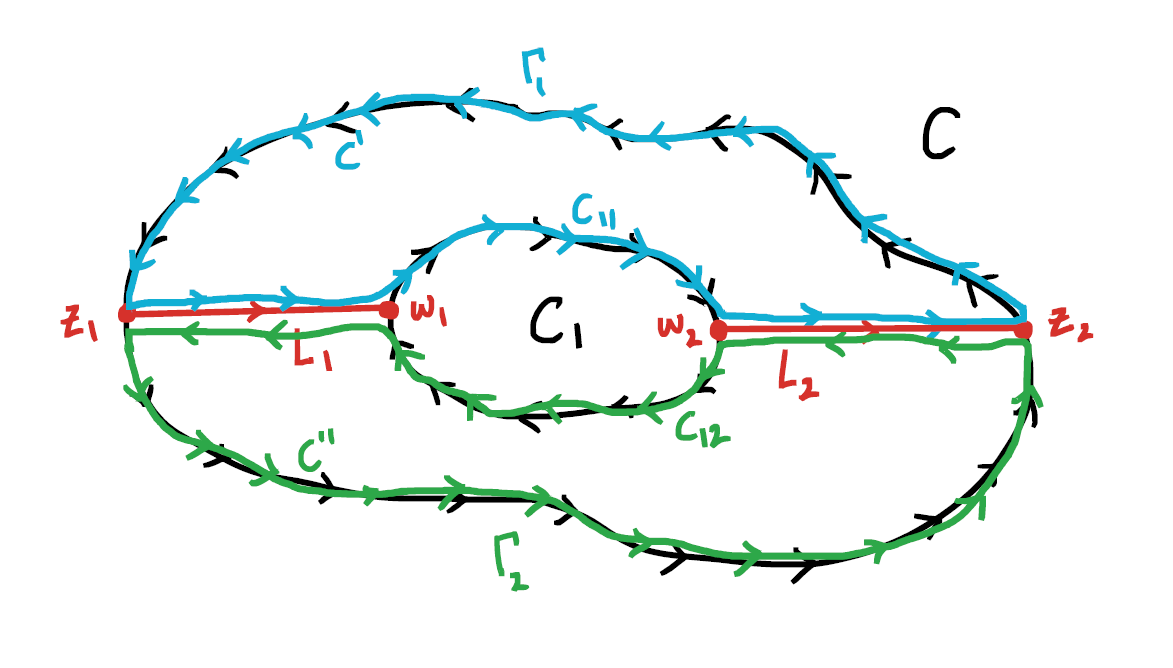
\includegraphics[scale=0.4]{Sections/Illustrations/CG-MCD-Base.png}
\end{center}
We note $C' + C'' = C$ and $C_{11} + C_{12} = C$.\\
\\
Then $f$ is holomorphic in the interior of and on the simple closed curves $\Gamma_1$ and $\Gamma_2$, so by Theorem \ref{cgthm} we have
\[\int_{\Gamma_1}f(z)\ dz = \int_{\Gamma_2}f(z)\ dz = 0\]
So, this gives us
\begin{align*}
0 &= \int_{\Gamma_1}f(z)\ dz + \int_{\Gamma_2}f(z)\ dz\\[1em]
 &= \left(\int_{L_1}f(z)\ dz + \int_{C_{11}}f(z)\ dz + \int_{L_2}f(z)\ dz + \int_{C'}f(z)\ dz\right)\\[1em]
 &\qquad + \left(-\int_{L_2}f(z)\ dz + \int_{C_{12}}f(z)\ dz - \int_{L_1}f(z)\ dz + \int_{C''}f(z)\ dz\right)\\[1em]
 &= \int_{C'}f(z)\ dz + \int_{C''}f(z)\ dz + \int_{C_{11}}f(z)\ dz + \int_{C_{12}}f(z)\ dz\\[1em]
 &= \int_{C}f(z)\ dz + \int_{C_1}f(z)\ dz
\end{align*}
\emph{Inductive Step.} Assume the statement holds for $n = k$, that is
\[\int_C\,f(z)\ dz + \sum_{i=1}^k\int_{C_i}f(z)\ dz = 0\]
for any $k$-many contours satisfying the hypotheses.\\
\\
Now, let $C_1,\ldots,C_k,C_{k+1}$ be any $k+1$-many contours. Introduce a polygon line $L$ that separates $C_1,\ldots,C_k$ from $C_{k+1}$, say with end points $z_1$ and $z_2$. We define $\Gamma_1$ and $\Gamma_2$ as follows.
\begin{itemize}
\item[$\Gamma_1$:] Start with $z_1$ and follow to $z_2$ along $C$ (we'll call this $C'$), then $z_2$ to $z_1$ along $-L$. So, 
\[\Gamma_1 = C' - L\]
\item[$\Gamma_2$:] Start with $z_1$ and follow to $z_2$ along $L$, then $z_2$ to $z_1$ along $C$ (we'll call this $C''$). So, 
\[\Gamma_2 = C'' + L\]
\end{itemize}
We note $C' + C'' = C$.
\begin{center}
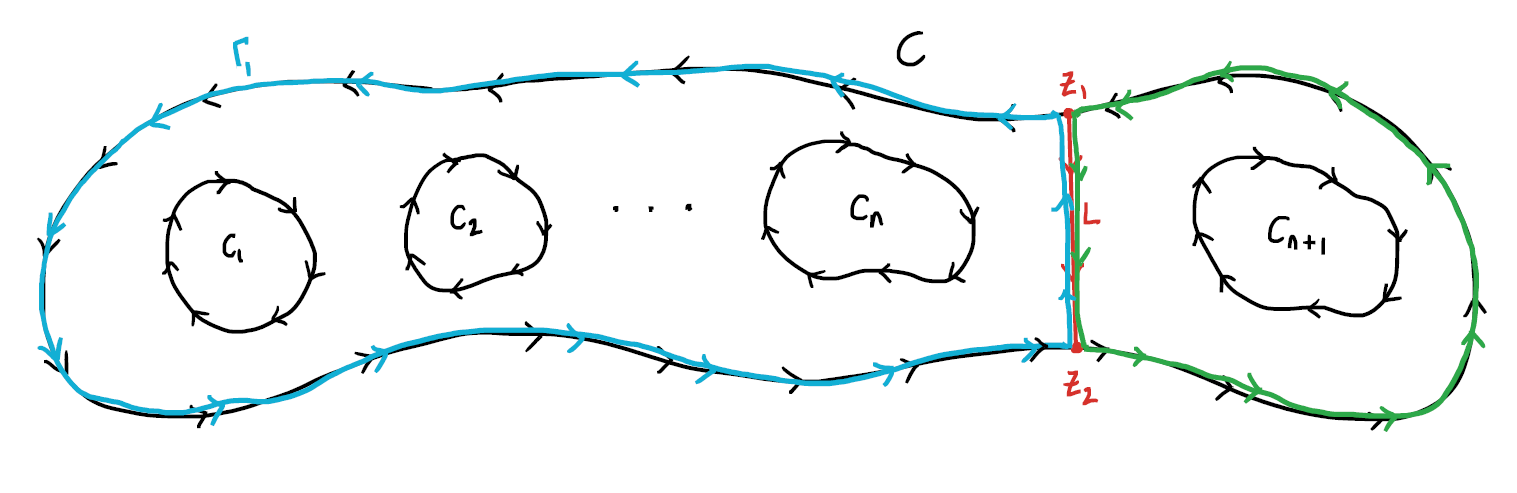
\includegraphics[scale=0.5]{Sections/Illustrations/CG-MCD-Induction.png}
\end{center}
We note that
\begin{align*}
\int_{\Gamma_1}f(z)\ dz + \int_{\Gamma_2}f(z)\ dz &= \left(\int_{C'}f(z)\ dz - \int_{L}\,f(z)\ dz\right) + \left(\int_{C''}f(z)\ dz + \int_{L}\,f(z)\ dz\right)\\[1em]
 &= \int_{C'}f(z)\ dz + \int_{C''}f(z)\ dz\\[1em]
 &= \int_C\,f(z)\ dz \tag{$\dagger$}
\end{align*}
By the inductive hypothesis
\[\int_{\Gamma_1}\,f(z)\ dz + \sum_{i=1}^k\int_{C_i}f(z)\ dz = 0\tag{1}\]
and by the computation in the base case we have
\[\int_{\Gamma_2}\,f(z)\ dz + \int_{C_{k+1}}f(z)\ dz = 0\tag{2}\]
Adding (1) and (2) and using ($\dagger$) we have
\[0 = \int_{\Gamma_1}\,f(z)\ dz + \sum_{i=1}^k\int_{C_i}f(z)\ dz + \int_{\Gamma_2}\,f(z)\ dz + \int_{C_{k+1}}f(z)\ dz = \int_C\,f(z)\ dz + \sum_{i=1}^{k+1}\int_{C_i}f(z)\ dz\]
Thus, we have proved our result using the principle of mathematical induction. 
\end{proof}

\medskip

\begin{corollary}[Principle of Deformation of Paths]\label{deformation}
Suppose $C_1$ and $C_2$ are positively oriented simple closed contours with $C_1$ interior to $C_2$.
\[\begin{tikzpicture}[scale=0.6]
    \begin{scope}
    \draw[use Hobby shortcut,closed=true,fill=indigo,fill opacity=1/15,draw opacity=0]
	(3,3) .. (6,3) .. (3,-1) .. (-1,-2.5) .. (-2,-1.5) .. (-4,0) .. (-2,3) .. (-1,4.5) .. (2,5);
    \draw[use Hobby shortcut,closed=true,clockwise arrowsend,thick]
	(3,3) .. (6,3) .. (3,-1) .. (-1,-2.5) .. (-2,-1.5) .. (-4,0) .. (-2,3) .. (-1,4.5) .. (2,5);
	\draw[use Hobby shortcut,closed=true,fill=white,clockwise arrowsend,thick]
	(0,-1.5) .. (-1.75,0) .. (0,2.5) .. (2,0);
    \end{scope}
    \node[label=below:{$C_2$}](A) at (6.5,1) {};
    \node[label=below:{$C_1$}](A) at (0,0) {};
\end{tikzpicture}\]
If $f$ is holomorphic on the region consisting of $C_1$ and $C_2$ and all the points between them, then
\[\int_{C_1}f(z)\ dz = \int_{C_2}f(z)\ dz\]
\end{corollary}
\begin{proof}
Applying Theorem \ref{cgthmgen} to $C_2$ and $-C_1$, we get
\[\int_{C_2}f(z)\ dz + \int_{-C_1}f(z)\ dz = 0.\]
Therefore, 
\[\int_{C_1}f(z)\ dz = \int_{C_2}f(z)\ dz\]\\[-2em]
\end{proof}

\medskip

Among other things, the principle of deformation of paths is useful for integrating over complicated contours. Often, we can just replace this contour with a circle.
\begin{example}
Let $C$ be any simple closed contour whose interior contains $0$. We show that
\[\int_C\frac{1}{z}\ dz = 2\pi i.\]
Since $0$ is interior to $C$, we can choose an $\epsilon > 0$ small enough such that $C_\epsilon = C_\epsilon(0)$ is contained in the interior of $C$. The region containing $C$ and $C_\epsilon$ and points between them does not contain $0$, so $1/z$ is holomorphic there. By Corollary \ref{deformation},
\begin{align*}
\int_C\,f(z)\ dz &= \int_{C_\epsilon}f(z)\ dz\\[1em]
 &= \int_0^{2\pi}\frac{1}{\epsilon e^{it}}\,ie^{it}\ dt = \int_0^{2\pi}\,i\ dt = 2\pi i
\end{align*}
\end{example}

\medskip

\begin{definition}[Singularities]
Suppose $f$ is not holomorphic at $z_0$, but every neighbourhood of $z_0$ contains a point at which $f$ is holomorphic, then $z_0$ is called a \cdef{singular\ point} (or \cdef{singularity}) \emph{of $f$}.\\[1em]
\[\begin{tikzpicture}[scale=0.65]
    \draw[<->,thick] (-1,0)--(5,0);
	\draw[<->,thick] (0,-1)--(0,5);
	\filldraw[firebrick,fill opacity=1/10,dashed](3,3) circle (2.5);
    \fill (3,3) circle (2pt);
    \node[] at (2.65,2.65) {$z_0$};
	\filldraw[indigo,fill opacity=1/10,dashed](3.9,3.9) circle (0.95);
    \fill (3.9,3.9) circle (2pt);
    \node[] at (3.45,3.9) {\footnotesize$w$};
    \node[] (3) at (8.5,1) {\footnotesize\color{firebrick}$f$ is not holomorphic here};
    \node[] (1) at (7.75,5) {\footnotesize\color{indigo}$f$ is holomorphic here};
    \node[] (2) at (4.1,3.9) {};
    \node[] (4) at (4.5,2.3) {};
	\path[every node/.style={font=\sffamily\small},<-,>=stealth, thick,indigo]
    (2) edge[bend right] node [left] {} (1);
    \path[every node/.style={font=\sffamily\small},->,>=stealth, thick,firebrick]
    (3) edge[bend right] node [left] {} (4);
  \end{tikzpicture}\]
\end{definition}

\medskip

\begin{example}\hfill
\begin{itemize}
\item[(1)] $f(z) = \dfrac{1}{z}$ has a singularity at $0$.
\item[(2)] $f(z) = \abs{z}^2$ has no singular points, as $f$ is only differentiable at $0$ but is nowhere holomorphic.
\item[(3)] $f(z) = \dfrac{z^2 + 3}{(z + 1)(z^2 + 5)}$ has singularities at those $z$ where
\[(z + 1)(z^2 + 5) = 0.\]
That is, at $-1,\, i\sqrt{5}$ and $-i\sqrt{5}$.
\end{itemize}
\end{example}

\medskip

\begin{remark}
More generally, the generalised Generalised Cauchy-Goursat Theorem (Theorem \ref{cgthmgen}) and its Corollary \ref{deformation} provide a technique for integrating functions over contours whose interior contains singularities of that function. The idea is to introduce small circles around the singular points, and apply the theorem (or corollary). It is usually easy to integrate over a circle. 
\end{remark}

\bigskip

\subsection{Cauchy's Integral Formula}
%\begin{mdframed}
%\begin{center}
%{\Large Cauchy's Integral Formula}
%\end{center}
%\end{mdframed}

\begin{discussion}
Cauchy's Integral Formula is a remarkable theorem. It asserts that if a function is holomorphic inside and on $C$, a simple closed contour, then its values interior to $C$ are completely determined by its values on $C$. 
\end{discussion}

\medskip

\begin{theorem}[Cauchy's Integral Formula]\label{cintform}
Let $C$ be a simple closed contour, with positive orientation, and let $f$ be a function that is holomorphic at all points on and interior to $C$. The for any $z_0 \in \mathrm{int}(C)$, we have
\[f(z_0) = \frac{1}{2\pi i}\int_C\,\frac{f(z)}{z - z_0}\,dz\]
\end{theorem}
\begin{proof}
Our strategy is to show that for all $\epsilon > 0$, we get
\[\abs{\int_C\,\frac{f(z)}{z - z_0}\,dz - f(z)\cdot 2\pi i} < \epsilon\]
because then
\[\int_C\,\frac{f(z)}{z - z_0}\,dz - f(z)\cdot 2\pi i = 0\]
Let $\epsilon > 0$, and since, by assumption, $f$ is holomorphic on $z_0$, it's continuous on $z_0$. So, there exists a $\delta > 0$ such that
\[\text{if }\ \abs{z - z_0} < \delta,\quad \text{then }\ \abs{f(z) - f(z_0)} < \frac{\epsilon}{2\pi}\]
Let $\rho > 0$ be small enough such that the circle $C_\rho = C_\rho(z_0)$ centered at $z_0$ of radius $\rho$ lies in the interior of $C$; assume $C_\rho$ has positive orientation. 
\[\begin{tikzpicture}[scale=0.6]
    \begin{scope}
    \draw[use Hobby shortcut,closed=true,fill=indigo,fill opacity=1/15,draw opacity=0]
	(3,3) .. (6,3) .. (3,-1) .. (-1,-2.5) .. (-2,-1.5) .. (-4,0) .. (-2,3) .. (-1,4.5) .. (2,5);
    \draw[use Hobby shortcut,closed=true,clockwise arrowsend]
	(3,3) .. (6,3) .. (3,-1) .. (-1,-2.5) .. (-2,-1.5) .. (-4,0) .. (-2,3) .. (-1,4.5) .. (2,5);
	\draw[use Hobby shortcut,closed=true,fill=white,clockwise arrowsend]
	(0,-1.5) .. (-1.5,0) .. (0,1.5) .. (1.5,0);
    \end{scope}
    \node[label=below:{$C$}](A) at (6.5,1) {};
    \draw [fill=black] (0,0) circle (2pt);
    \node[label=below:{$z_0$}](A) at (0,0) {};
    \draw[](0,0)--(1.3,0.748) node[sloped,midway,above]{\footnotesize $\rho$};
\end{tikzpicture}\]
We may assume $\rho < \delta$, then for every point $z \in C_\rho$, since $\abs{z - z_0} = \rho < \delta$, we have
\[\abs{f(z) - f(z_0)} < \frac{\epsilon}{2\pi},\quad \text{therefore }\ \max_{z \in C_\rho}\abs{f(z) - f(z_0)} < \frac{\epsilon}{2\pi}\]
Now, note that 
\[\frac{f(z)}{z - z_0}\]
is holomorphic on the region consisting of $C,\,C_\rho$ and all points that are interior to $C$ but exterior to $C_\rho$. So, by Corollary \ref{deformation}, we have
\[\int_C\,\frac{f(z)}{z - z_0}\,dz = \int_{C_\rho}\,\frac{f(z)}{z - z_0}\,dz\]
and then
\begin{align*}
\abs{\int_C\,\frac{f(z)}{z - z_0}\,dz - f(z)\cdot 2\pi i} &= \abs{\int_{C_\rho}\frac{f(z)}{z - z_0} - f(z)\cdot 2\pi i}\\[1em]
 &= \abs{\int_{C_{\rho}}\frac{f(z)}{z - z_0} - f(z)\int_{C_{\rho}}\,\frac{1}{z - z_0}\,dz}\\[1em]
 &= \abs{\int_{C_{\rho}}\frac{f(z) - f(z_0)}{z - z_0}\,dz}\\[1em]
 &\leq \max_{z \in C_{\rho}}\abs{\frac{f(z) - f(z_0)}{z - z_0}}\cdot L(C_{\rho})\\[1em]
 &= \max_{z \in C_{\rho}}\frac{\abs{f(z) - f(z_0)}}{\rho}\cdot (2\pi\rho)\\[1em]
 &= \frac{1}{\rho}\max_{z \in C_{\rho}}\abs{f(z) - f(z_0)}\cdot (2\pi\rho)\\[1em]
 &< \frac{\epsilon}{2\pi}\cdot 2\pi\\[1em]
 &= \epsilon
\end{align*}
and the claim follows.
\end{proof}

\medskip

Among other things, Cauchy's Integral formula is useful for computing integrals. 
\begin{example}\lecmargin{26}\hfill
\begin{itemize}[itemsep=2em]
\item[(1)] Let's compute $\displaystyle \int_C\, \frac{\cos z}{z(z^2 + 2)}\, dz$, where $C$ is the unit circle, positively oriented.\\
\\
Consider
\[f(z) = \frac{\cos z}{z^2 + 2}\]
Then $f$ is holomorphic on all points on and interior to $C$, as they don't include $\pm 2i$ and $0$ is in the interior or $C$. Therefore, by Cauchy's Integral Formula (Theorem \ref{cintform}) we have
\[\int_C\, \frac{\cos z}{z(z^2 + 2)}\, dz = \int_C\, \frac{f(z)}{z - 0}\, dz = 2\pi i\cdot f(0) = \pi i.\]

\item[(2)] Let's compute $\displaystyle \int_C\, \frac{e^{z^2}}{z - 1}\, dz$, where $C$ is a positively oriented circle with radius $2$.\\
\\
Consider $f(z) = e^{z^2}$, then $f$ is entire, and therefore holomorphic on all points on and interior to $C$. Therefore, by Cauchy's Integral Formula (Theorem \ref{cintform}) we have
\[\int_C\, \frac{e^{z^2}}{z - 1}\, dz = 2\pi if(1) = 2\pi ie.\]

\item[(3)] Let's compute $\displaystyle \int_C\, \frac{z^2 + 1}{z^2 - 1}\, dz = \int_C\, \frac{z^2 + 1}{(z - 1)(z + 1)}\, dz$, where $C$ is as follows
\begin{center}
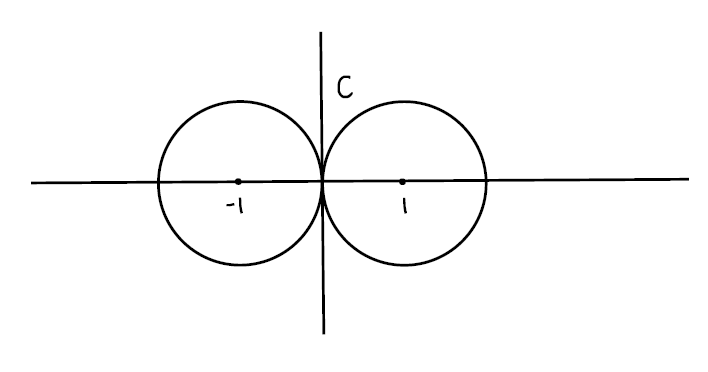
\includegraphics[scale=0.75]{Sections/Illustrations/Example-3.10.3-3-curve.png}
\end{center}
The contour $C$ is not simple but it can be decomposed as a sum of simple closed contours $C = C_1 - C_2$
\begin{center}
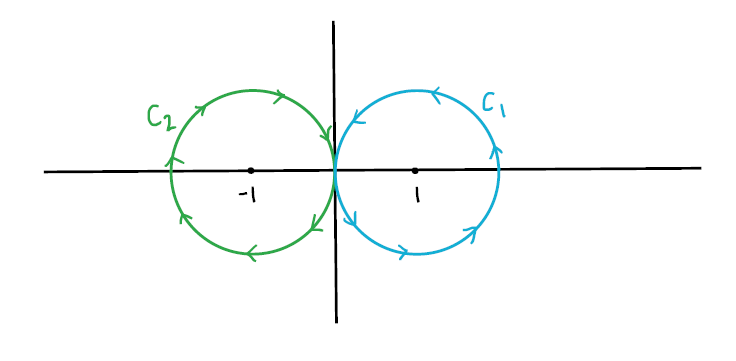
\includegraphics[scale=0.75]{Sections/Illustrations/Example-3.10.3-3-contour.png}
\end{center}
So, 
\[\int_C\, \frac{z^2 + 1}{(z - 1)(z + 1)}\,dz = \int_{C_1}\, \frac{z^2 + 1}{(z - 1)(z + 1)}\,dz - \int_{C_2}\, \frac{z^2 + 1}{(z - 1)(z + 1)}\,dz\]
For $C_1$, consider
\[f(z) = \frac{z^2 + 1}{z + 1},\]
then $f$ is holomorphic on all points on and interior to $C_1$, as they don't include $-1$, and $1$ is in the interior or $C_1$. Therefore by Cauchy's Integral Formula (Theorem \ref{cintform}) we have
\[\int_{C_1}\, \frac{z^2 + 1}{(z - 1)(z + 1)}\,dz = \int_{C_1}\, \frac{f(z)}{z - 1}\,dz = 2\pi i\cdot f(1) = 2\pi i\]
For $C_2$, consider
\[g(z) = \frac{z^2 + 1}{z - 1},\]
then $g$ is holomorphic on all points on and interior to $C_2$, as they don't include $1$, and $-1$ is in the interior or $C_2$. Therefore by Cauchy's Integral Formula (Theorem \ref{cintform}) we have
\[\int_{C_2}\, \frac{z^2 + 1}{(z - 1)(z + 1)}\,dz = \int_{C_2}\, \frac{g(z)}{z + 1}\,dz = 2\pi i\cdot g(-1) = -2\pi i\]
Hence, 
\[\int_C\, \frac{z^2 + 1}{(z - 1)(z + 1)}\,dz = \int_{C_1}\, \frac{z^2 + 1}{(z - 1)(z + 1)}\,dz - \int_{C_2}\, \frac{z^2 + 1}{(z - 1)(z + 1)}\,dz = 2\pi i + 2\pi i = 4\pi i.\]
\end{itemize}
\end{example}

\medskip

\begin{theorem}[Generalised Cauchy's Integral Formula]\label{gencintform}
Let $C$ be a simple closed contour, with positive orientation, and let $f$ be a function that is holomorphic at all points on and interior to $C$. The for any $z_0 \in \mathrm{int}(C)$, we have that $f^{(n)}(z_0)$ exists and
\[f^{(n)}(z_0) = \frac{n!}{2\pi i}\int_C\,\frac{f(z)}{(z - z_0)^{n+1}}\,dz\]
\end{theorem}
\begin{proof}
We prove by induction, with the base case $n = 0$ being just Theorem \ref{cintform}. Assume the statements holds for $n = k$, we need to prove  that
\[f^{(k+1)}(z_0) \coloneqq \lim_{h \to 0}\frac{f^{(k)}(z_0 + h) - f^{(k)}(z_0)}{h} = \frac{(k+1)!}{2\pi i}\int_C\,\frac{f(z)}{(z - z_0)^{(k+1)+1}}\,dz\]
We assume $\abs{h}$ is small enough such that $z + h \in \mathrm{int}(C)$, then by the inductive hypothesis
\begin{align*}
f^{(k)}(z_0 + h) &= \frac{k!}{2\pi i}\int_C\,\frac{f(z)}{(z - (z_0 + h))^{k+1}}\,dz\\[1em]
f^{(k)}(z_0) &= \frac{k!}{2\pi i}\int_C\,\frac{f(z)}{(z - z_0)^{k+1}}\,dz
\end{align*}
Recall the algebraic identity, that for $a,\,b \in \cc$ we have
\[a^{k+1} - b^{k+1} = (a - b)(a^k + a^{k-1}b + \cdots + ab^{k-1} + b^k),\]
We will apply this to $a = \dfrac{1}{z - z_0 - h}$ and $b = \dfrac{1}{z - z_0}$, and we also note $\lim_{h \to 0}a = b$. Then,
\begin{align*}
\lim_{h \to 0}&\,\frac{f^{(k)}(z_0 + h) - f^{(k)}(z_0)}{h}\\[1em]
&= \lim_{h \to 0}\,\frac{k!}{2\pi i}\int_C\,\frac{f(z)}{h}\left(\frac{1}{(z - z_0 - h)^{k+1}} - \frac{1}{(z - z_0)^{k+1}}\right)\,dz\\[1em]
 &= \lim_{h \to 0}\,\frac{k!}{2\pi i}\int_C\,\frac{f(z)}{h}\left(\frac{1}{z - z_0 - h} - \frac{1}{z - z_0}\right)(a^k + a^{k-1}b + \cdots + ab^{k-1} + b^k)\,dz \\[1em]
 &= \lim_{h \to 0}\,\frac{k!}{2\pi i}\int_C\,\frac{f(z)}{h}\left(\frac{h}{(z - z_0 - h)(z - z_0)}\right)(a^k + a^{k-1}b + \cdots + ab^{k-1} + b^k)\,dz%\\[1em]
\end{align*}
\begin{align*}
 \phantom{\lim_{h \to 0}} &= \lim_{h \to 0}\,\frac{k!}{2\pi i}\int_C\,\left(\frac{f(z)}{(z - z_0 - h)(z - z_0)}\right)(a^k + a^{k-1}b + \cdots + ab^{k-1} + b^k)\,dz \\[1em]
 &= \frac{k!}{2\pi i}\int_C\,\lim_{h \to 0}\,\left(\frac{f(z)}{(z - z_0 - h)(z - z_0)}\right)(a^k + a^{k-1}b + \cdots + ab^{k-1} + b^k)\,dz \\[1em]
 &= \frac{k!}{2\pi i}\int_C\,\left(\frac{f(z)}{(z - z_0)^2}\right)(b^k + b^{k-1}b + \cdots + b\cdot b^{k-1} + b^k)\,dz\\[1em]
 &= \frac{k!}{2\pi i}\int_C\,\frac{f(z)}{(z - z_0)^2}\cdot(k+1)\cdot b^k\,dz \\[1em]
 &= \frac{(k+1)!}{2\pi i}\int_C\,\frac{f(z)}{(z - z_0)^2}\cdot\frac{1}{(z - z_0)^k}\,dz \\[1em]
 &= \frac{(k+1)!}{2\pi i}\int_C\,\frac{f(z)}{(z - z_0)^{(k+1)+1}}\,dz 
\end{align*}
Thus we have our result by the principle of mathematical induction. 
\end{proof}

\medskip

\begin{example}
Compute the integral
\[\frac{1}{2\pi i}\int_C\,\frac{(1 + z)^n}{z^{k+1}}\,dz\]
where $C$ is any simple closed positively oriented contour whose interior contains $0$ and $0 \leq k \leq n$.\\
\\
Let $f(z) = (1 + z)^n$, since $f$ is entire, $f$ is holomorphic on all points on and interior to $C$. Since $0$ is in the interior of $C$, then generalised Cauchy's Integral formula (Theorem \ref{gencintform}) gives us
\begin{align*}
\frac{1}{2\pi i}\int_C\,\frac{(1 + z)^n}{z^{k+1}}\,dz &= \frac{1}{k!}\left(\frac{k!}{2\pi i}\int_C\,\frac{(1 + z)^n}{(z - 0)^{k+1}}\,dz\right) = \frac{1}{k!}\cdot f^{(k)}(0)
\end{align*}
We have, 
\[f^{(k)}(z) = n(n-1)\cdots (n-(k-1))(1 + z)^{n-k},\]
and therefore
\[f^{(k)}(0) = n(n-1)\cdots (n-(k-1)) = \frac{n!}{(n-k)!}\]
Hence, 
\[\frac{1}{2\pi i}\int_C\,\frac{(1 + z)^n}{z^{k+1}}\,dz = \frac{1}{k!}\cdot f^{(k)}(0) = \frac{n!}{k!(n-k)!} = \binom{n}{k}\]
\end{example}

\medskip

\begin{theorem}[Derivatives of Holomorphic functions are Holomorphic]\label{holsmooth}
Suppose that $f$ is holomorphic at $z_0 \in \cc$, then for all $n\in \zz_{>0}$, $f^{(n)}$ is also holomorphic at $z_0$. 
\end{theorem}
\begin{proof}
Suppose $f$ is holomorphic at $z_0 \in \cc$. Choose an open disk $D_\epsilon(z_0)$ on which $f$ is differentiable. To conclude $f'$ exists and is holomorphic at $z_0$, it's enough to find a neighbourhood of $z_0$ where $f''(w)$ exists for all $w$ in that neighbourhood. Let $C$ be the positive oriented circle of radius $\epsilon/2$ centered at $z_0$, then $f$ is holomorphic on all points on and interior to $C$. So, by generalised Cauchy's Integral formula (Theorem \ref{gencintform}),
\[f''(w) = \frac{2!}{2\pi i}\int_C\,\frac{f(z)}{(z - w)^3}\,dz\]
for any $w$ in the interior of $C$. Thus, $f'$ is differentiable in the open set $D_{\epsilon/2}(z_0)$, and hence $f'$ is holomorphic at $z_0$. Induction then gives us that $f^{(n)}$ is holomorphic at $z_0$ for any $n\in \zz_{>0}$.
\end{proof}

\medskip

\begin{corollary}
If $f(z) = u(x,y) + iv(x,y)$ is holomorphic at $z = x + iy$, then $u$ and $v$ have continuous partial derivatives of all orders at $(x,y)$. 
\end{corollary}

\medskip

\begin{theorem}[Morera's Theorem]\label{morera}\lecmargin{27}
Suppose $f$ is continuous on a domain $G$. If
\[\int_C\,f(z)\,dz = 0\]
for every closed contour $C \subseteq G$, then $f$ is holomorphic on $G$. 
\end{theorem}
\begin{proof}
By Theorem \ref{FTCoCI}, there exists a holomorphic function $F:G \to \cc$ such that $F'(z) = f(z)$ for all $z \in G$. But by Theorem \ref{holsmooth}, $F'$ is holomorphic on $G$, and therefore so is $f$. 
\end{proof}

\medskip

\begin{remark}
When $G$ is simply connected, Morera's theorem (Theorem \ref{morera}) is just the converse of Cauchy-Goursat Theorem for simply connected domains (Theorem \ref{cgthmsc}).
\end{remark}

\medskip

\begin{theorem}[Cauchy's Inequalities]\label{cauchyineq}
Suppose that $f$ is holomorphic on all points on and interior to $C_R = C_R(z_0)$, a positively oriented circle of radius $R$ centered at some $z_0 \in \cc$. Then,
\[|f^{(n)}(z_0)| \leq \frac{n!}{R^n}\,\max_{z \in C_R(z_0)}\abs{f(z)}\]
\end{theorem}
\begin{proof}
By Theorem \ref{gencintform}, 
\[f^{(n)}(z_0) = \frac{n!}{2\pi i}\int_{C_R}\,\frac{f(z)}{(z - z_0)^{n+1}}\,dz\]
Hence, 
\begin{align*}
|f^{(n)}(z_0)|= \abs{\frac{n!}{2\pi i}\int_{C_R}\,\frac{f(z)}{(z - z_0)^{n+1}}\,dz} &= \frac{n!}{2\pi i}\abs{\int_{C_R}\,\frac{f(z)}{(z - z_0)^{n+1}}\,dz}\\[1em]
&\leq \frac{n!}{2\pi i}\max_{z \in C_R}\,\abs{\frac{f(z)}{(z - z_0)^{n+1}}}\cdot L(C_R)\\[1em]
&= \frac{n!}{2\pi i}\max_{z \in C_R}\,\frac{\abs{f(z)}}{R^{n+1}}\cdot 2\pi R\\[1em]
&= \frac{n!}{R^n}\,\max_{z \in C_R}\abs{f(z)}\\[-2.5em]
\end{align*}
\end{proof}

\bigskip

\subsection{Liouville's Theorem and the Fundamental Theorem of Algebra}
%\begin{mdframed}
%\begin{center}
%{\Large Liouville's Theorem and the Fundamental Theorem of Algebra}
%\end{center}
%\end{mdframed}
As an application, we will prove that every non-constant polynomial with complex coefficients has a root in $\cc$. In the language of algebra, we will provide a proof for the fact that $\cc$ is \emph{algebraically closed}. Thus, the the statement is ``purely algebraic" while no ``purely algebraic" proof exists. The proof relies on the following wonderful theorem. 

\medskip

\begin{theorem}[Liouville's Theorem]\label{liouville}
Every bounded entire function is constant. 
\end{theorem}
\begin{proof}
We show that $f'(z) = 0$ for all $z \in \cc$, then it follows that $f$ is constant since $\cc$ is a domain by Theorem \ref{der0const}.\\
\\
Consider any $z_0 \in \cc$. Since $f$ is bounded, we can find a $M>0$ such that $\abs{f(z)} \leq M$ for all $z \in \cc$. Let $C_R(z_0)$ be a circle of radius $R$ centered at $z_0$, then $f$ is holomorphic at all points on and interior to $C_R(z_0)$. Hence, by Theorem \ref{cauchyineq},
\begin{align*}
\abs{f'(z_0)} &\leq \frac{1}{R}\max_{z \in C_R(z_0)}\abs{f(z)}\\[0.5em]
&\leq \frac{M}{R} \to 0,\ \text{ as } R \to \infty
\end{align*}
Thus $\abs{f'(z_0)} = 0$, giving us $f'(z_0) = 0$. Since $z_0$ was arbitrary, the result follows. 
\end{proof} 

\medskip

\begin{theorem}[Fundamental Theorem of Algebra]
For any polynomial $p(z) = a_0 + a_1z + \cdots + a_nz^n$ where $a_n \neq 0,\ a_i \in \cc$ and $n \geq 1$, there exists an $\alpha \in \cc$ such that $p(\alpha) = 0$. That is, every non-constant polynomial $p(z)$ has at least one root in $\cc$. 
\end{theorem}
\begin{proof}
Suppose otherwise that $p(z)$ has no root in $\cc$, then $p(z) \neq 0$ for every $z \in \cc$. Hence $1/p(z)$ is an entire function. We show that $1/p(z)$ is bounded.\\
\\
For a non-zero $z \in \cc$, consider the complex number
\[w_z \coloneqq \frac{a_0}{z^n} + \frac{a_1}{z^{n-1}} + \cdots + \frac{a_{n-1}}{z}\]
Note that $p(z) = (w_z + a_n)\ z^n$, and by triangle inequality we have
\[\abs{w_z} \leq \frac{\abs{a_0}}{\abs{z}^n} + \frac{\abs{a_1}}{\abs{z}^{n-1}} + \cdots + \frac{\abs{a_{n-1}}}{\abs{z}} = \sum_{k=0}^{n-1}\frac{\abs{a_k}}{\abs{z}^{n-k}}\]
For each $0 \leq k \leq n-1$ we note that $\dfrac{\abs{a_k}}{\abs{z}^{n-k}} \to 0$ as $z \to \infty$.\\[0.5em]
Then, for $\epsilon = \dfrac{\abs{a_n}}{2n} > 0$, we can find an $R > 0$ such that whenever $\abs{z} > R$, we get
\[\frac{\abs{a_k}}{\abs{z}^{n-k}} = \abs{\frac{\abs{a_k}}{\abs{z}^{n-k}} - 0} < \epsilon = \frac{\abs{a_n}}{2n}\]
for any $k = 0,\ldots,n-1$. This then gives us
\[\abs{w_z} \leq \sum_{k=0}^{n-1}\frac{\abs{a_k}}{\abs{z}^{n-k}} < \sum_{k=0}^{n-1}\frac{\abs{a_n}}{2n} = n\cdot \frac{\abs{a_n}}{2n} = \frac{\abs{a_n}}{2}\]
Now, by the reverse triangle inequality we have
\[\abs{a_n + w_z} \geq \abs{\abs{a_n} - \abs{w_z}} > \abs{\abs{a_n} - \frac{\abs{a_n}}{2}} = \frac{\abs{a_n}}{2}\]
Thus, 
\begin{align*}
\abs{p(z)} &= \abs{(w_z + a_n)\ z^n}\\[0.5em]
&= \abs{w_z + a_n}\abs{z^n} > \frac{\abs{a_n}}{2}R^n
\end{align*}
Therefore, for any $z \in \cc$ such that $\abs{z} > R$, we have
\[\abs{\frac{1}{p(z)}} \leq \frac{2}{R^n\abs{a_n}}\]
So, $1/p(z)$ is bounded outside the closed disk $\overline{D}_R(0)$.\\[0.5em]
Now, the closed disk $\overline{D}_R(0)$ is compact (closed and bounded) and $1/p(z)$ is continuous on $\overline{D}_R(0)$. Hence $1/p(z)$ is bounded on $\overline{D}_R(0)$ by Theorem \ref{evt}.\\
\\
Thus, $1/p(z)$ is bounded on all of $\cc$. Hence, by Theorem \ref{liouville}, $1/p(z)$ is constant, and therefore so is $p(z)$. We have arrived a contradiction, since $p(z)$ was non-constant by assumption. 
\end{proof}

\medskip

\begin{lemma}[Maximum Modulus Principle]
Suppose that $\abs{f(z)} \leq \abs{f(z_0)}$ at each point $z$ in a neighbourhood $D_\epsilon(z_0)$ where $f$ is holomorphic. Then $f(z) = f(z_0)$ on $D_\epsilon(z_0)$. That is, if a holomorphic function on an open disk achieves its maximum on it, then it is constant on the open disk.
\end{lemma}
\begin{proof}
Let $z_1 \in D_\epsilon(z_0)$ such that $z_1 \neq z_0$. Set $\rho \coloneqq \abs{z_1 - z_0} > 0$, and consider $C_\rho = C_\rho(z_0)$, the circle of radius $\rho > 0$ centered at $z_0$, which is interior to $D_\epsilon(z_0)$. We parametrise $C_\rho$ as $z(t) = z_0 + \rho e^{it}$ for $0 \leq t \leq 2\pi$.
\begin{center}
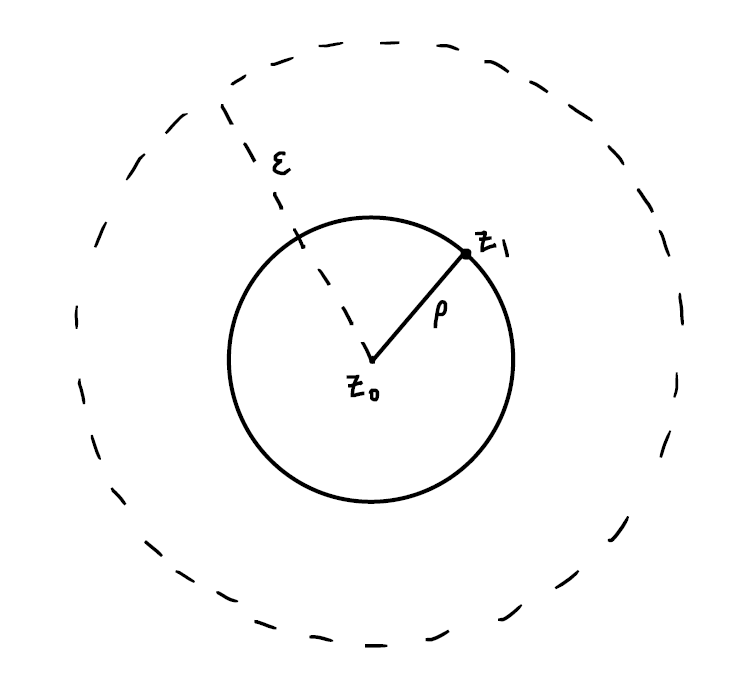
\includegraphics[scale=0.55]{Sections/Illustrations/MMP.png}
\end{center}
By Theorem \ref{cintform},
\begin{align*}
\abs{f(z_0)} = \abs{\frac{1}{2\pi i}\int_{C_\rho}\,\frac{f(z)}{z - z_0}\, dz} &= \frac{1}{2\pi}\abs{\int_{C_\rho}\,\frac{f(z)}{z - z_0}\, dz}\\[1em]
 &= \frac{1}{2\pi}\abs{\int_0^{2\pi}\,\frac{f(z_0 + \rho e^{it})}{\rho e^{it}}\,i\rho e^{it}\ dt}\\[1em]
 &= \frac{1}{2\pi}\abs{\int_0^{2\pi}\,f(z_0 + \rho e^{it})\ dt}\\[1em]
 &\leq \frac{1}{2\pi}\int_0^{2\pi}\,|f(z_0 + \rho e^{it})|\ dt\\[1em]
 &\leq \frac{1}{2\pi}\int_0^{2\pi}\,\abs{f(z_0)}\ dt,\quad \text{by assumption}\\[1em]
 &\leq \abs{f(z_0)}
\end{align*} 
This tells us that
\[\abs{f(z_0)} = \frac{1}{2\pi}\int_0^{2\pi}\,|f(z_0 + \rho e^{it})|\ dt \tag{$\dagger$}\]
Since, $\displaystyle f(z_0) =  \frac{1}{2\pi}\int_0^{2\pi}\,\abs{f(z_0)}\ dt$. Rewriting ($\dagger$), we have
\[\frac{1}{2\pi}\int_0^{2\pi}\, \abs{f(z_0)} - |f(z_0 + \rho e^{it})|\ dt = 0\]
By assumption $\abs{f(z_0)} - |f(z_0 + \rho e^{it})| \geq 0$; suppose $\abs{f(z_0)} - |f(z_0 + \rho e^{it})| > 0$, then necessarily 
\[\frac{1}{2\pi}\int_0^{2\pi}\, \abs{f(z_0)} - |f(z_0 + \rho e^{it})|\ dt > 0\tag{$*$}\]
since the integrand in ($*$) is continuous in the variable $t$, giving us a contradiction. Thus, 
\[\abs{f(z_0)} - |f(z_0 + \rho e^{it})| = 0\]
Therefore $\abs{f(z)} = \abs{f(z_0)}$ for every $z \in C_\rho(z_0)$. Varying the radius $\rho > 0$, we may then obtain $\abs{f(z)} = \abs{f(z_0)}$ for every $z \in D_\epsilon(z_0)$.\\
\\
Thus, $\abs{f}$ is a holomorphic function on $D_\epsilon(z_0)$, and thus by Corollary \ref{absholconst}, we have $f$ is constant on $D_\epsilon(z_0)$ and $f(z) = f(z_0)$ for every $z \in D_\epsilon(z_0)$.
\end{proof}